%appendix
\newpage
\appendix
\section{Results of training for one-dimensional self-organizing maps}
\label{app: high_Z_1d_soms}
As mentioned in Sec.~\ref{sec: 1D_somz}, we changed the size of the SOM from $1\times2$ to $1\times22$. In that section we show some example of the results; here we show the rest of the maps to monitor the changes in the map over various sizes.

\label{app: 1d}
    \begin{figure}
        \begin{subfigure}[b]{0.5\textwidth}
            \centering
            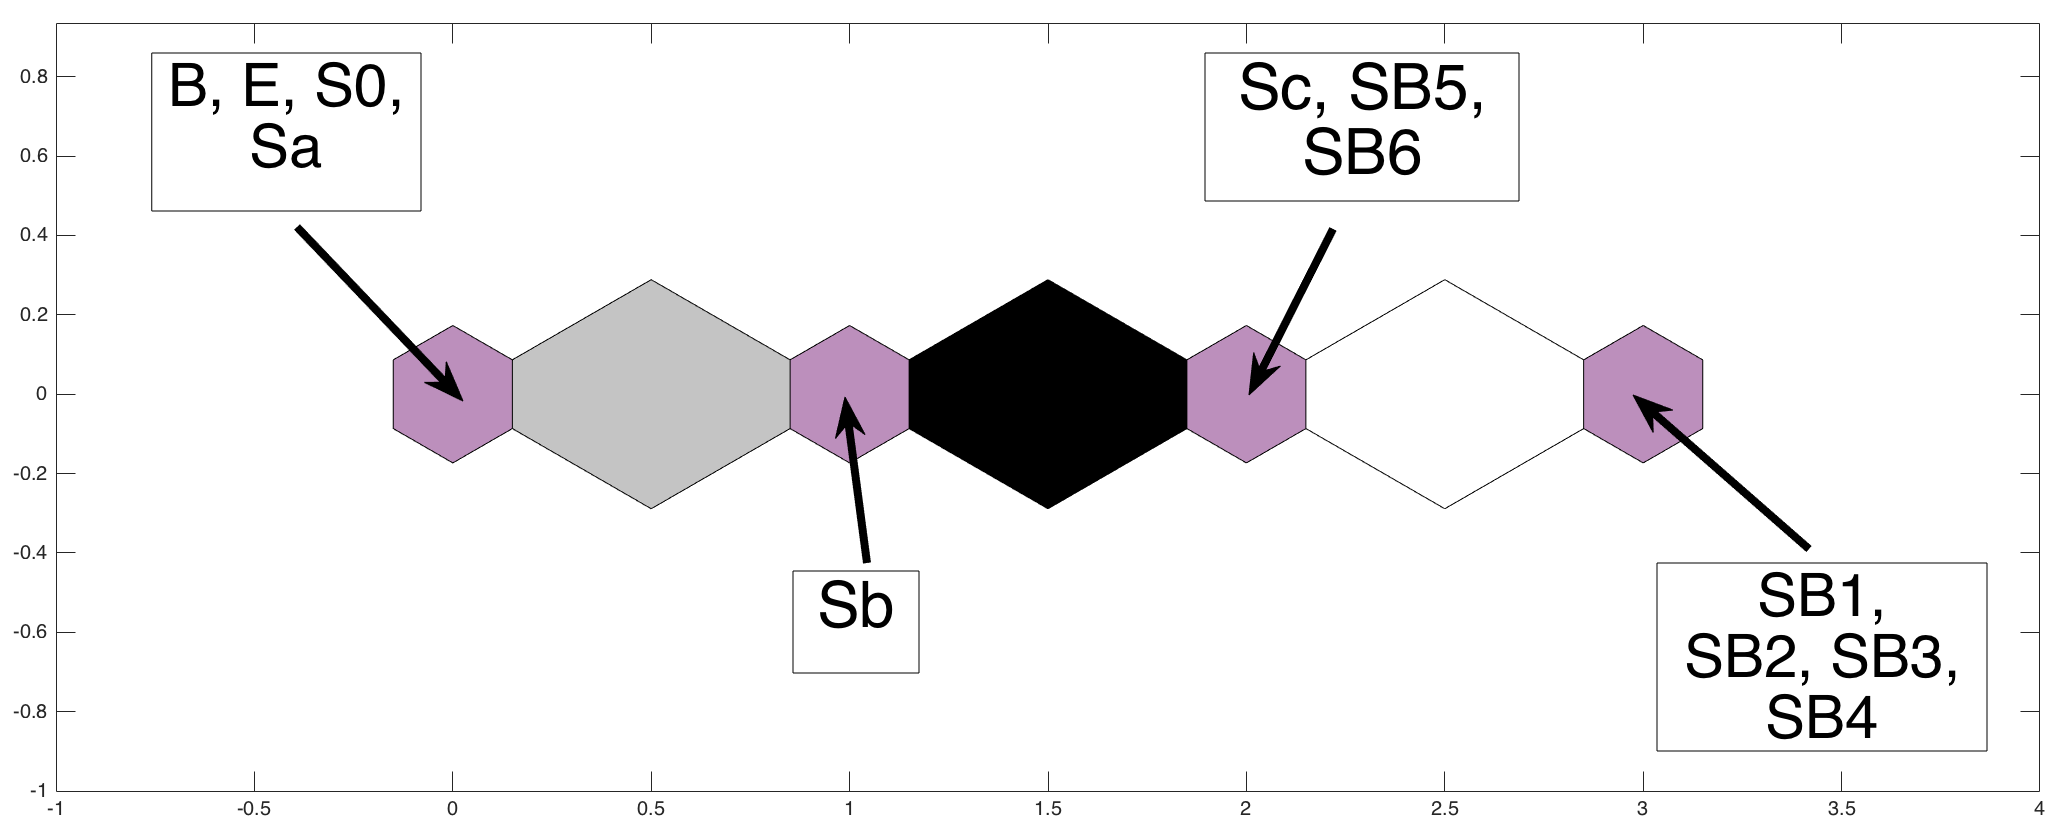
\includegraphics[width=\textwidth]{../images0.01/1d/apps/dist_1_by_4.png}
            %\caption{$1\times4$ weight map}
             %\label{fig: 1by4T}
        \end{subfigure}
        \hfill
        \begin{subfigure}[b]{0.5\textwidth}
             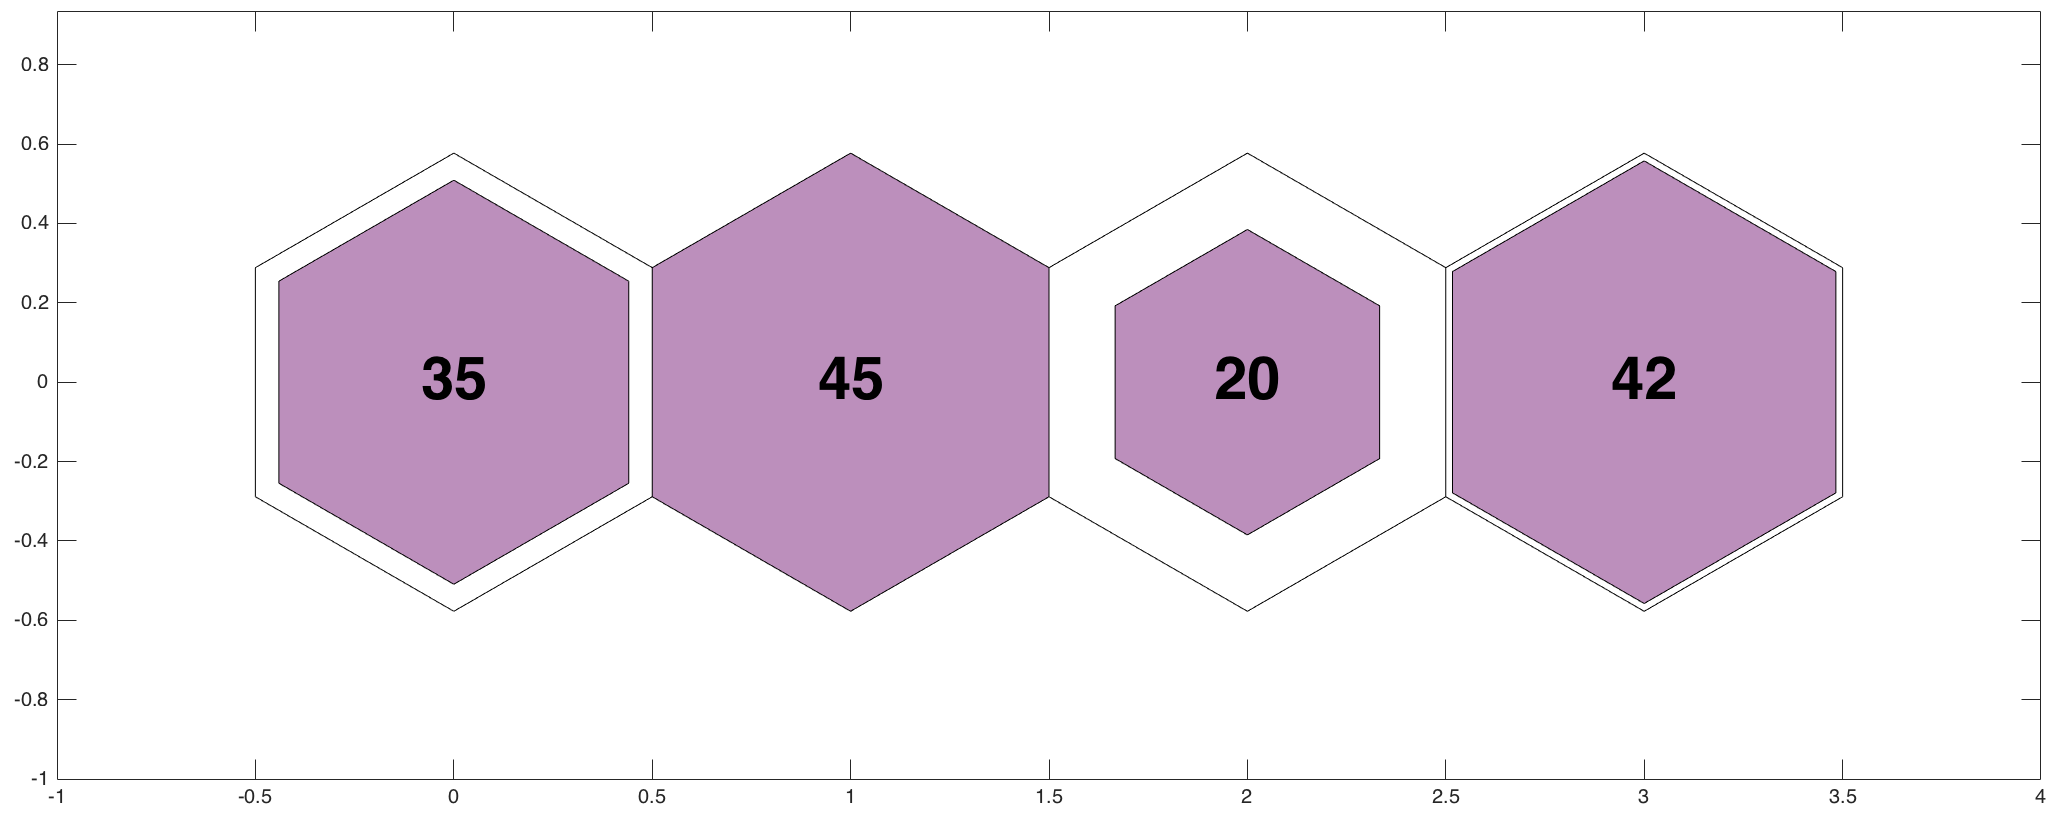
\includegraphics[width=\textwidth]{../images0.01/1d/apps/hit_v_1_by_4.png}
             %\caption{$1\times4$ hits map}
             %\label{fig: 1by4Thits}
        \end{subfigure}
                \caption{Results of training network in $1\times4$~grid.}
         \label{fig: 1by4T}
    \end{figure}
    
    \begin{figure}
        \begin{subfigure}[b]{0.5\textwidth}
            \centering
            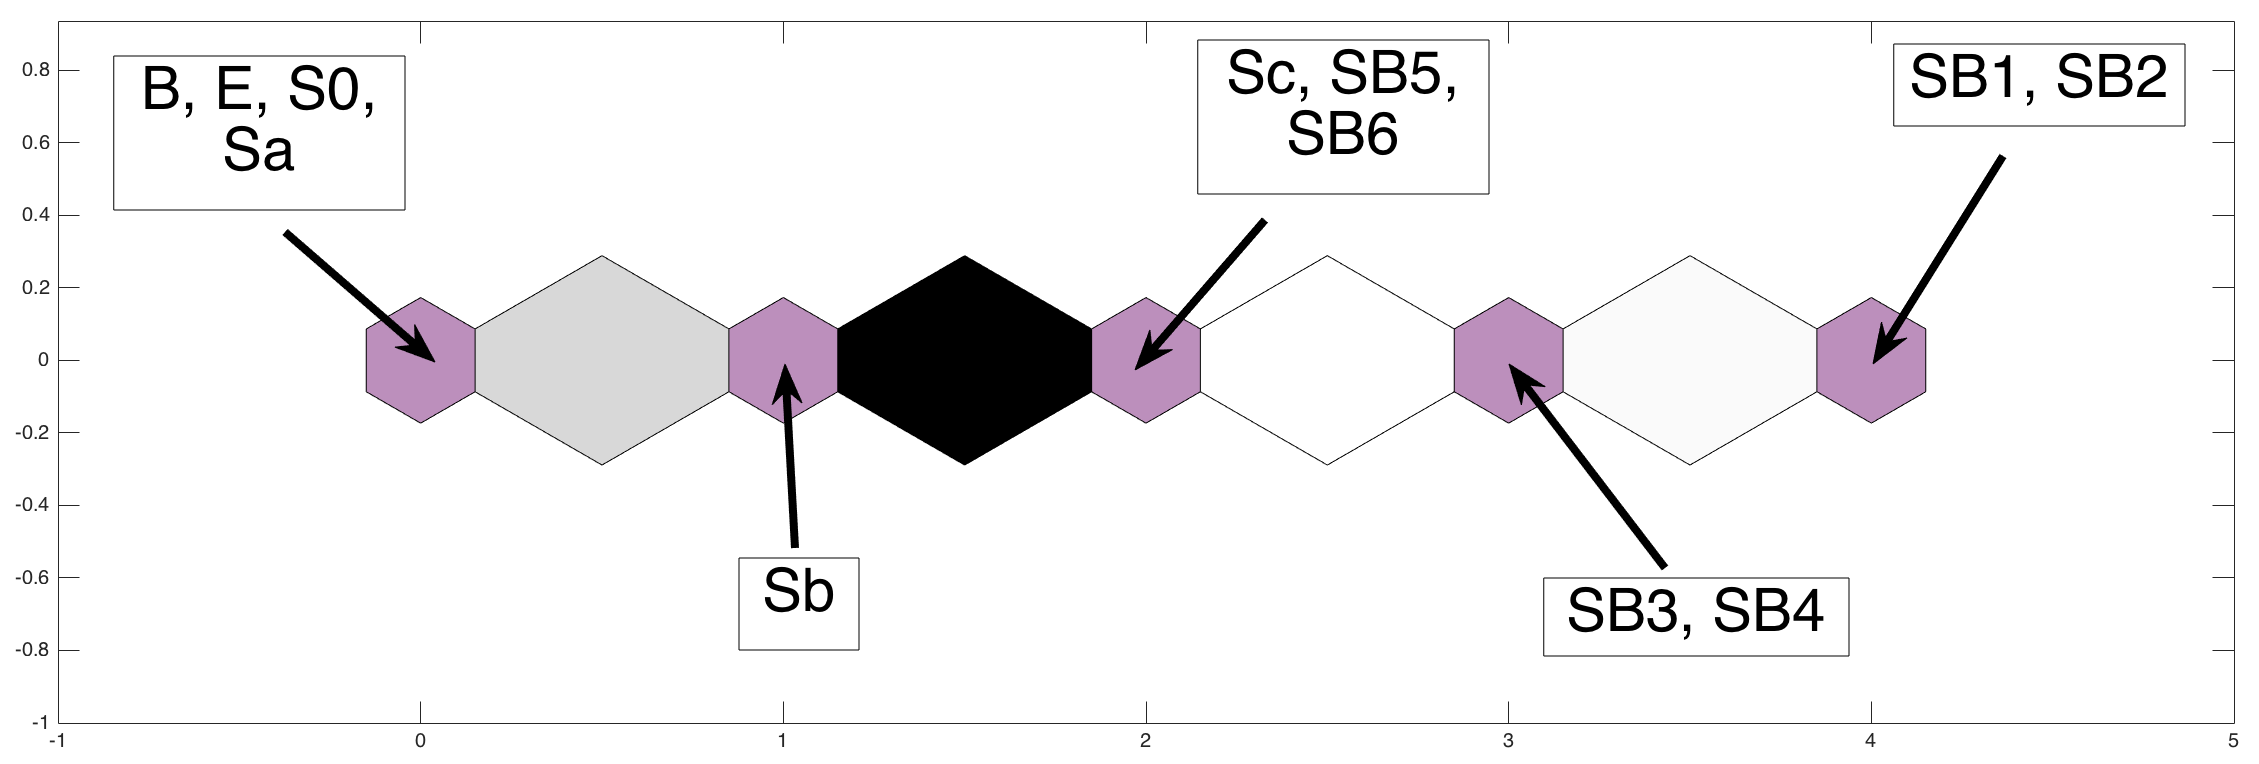
\includegraphics[width=\textwidth]{../images0.01/1d/apps/dist_1_by_5.png}
            %\caption{$1\times5$ weight map}
             %\label{fig: 1by5T}
        \end{subfigure}
        \hfill
        \begin{subfigure}[b]{0.5\textwidth}
             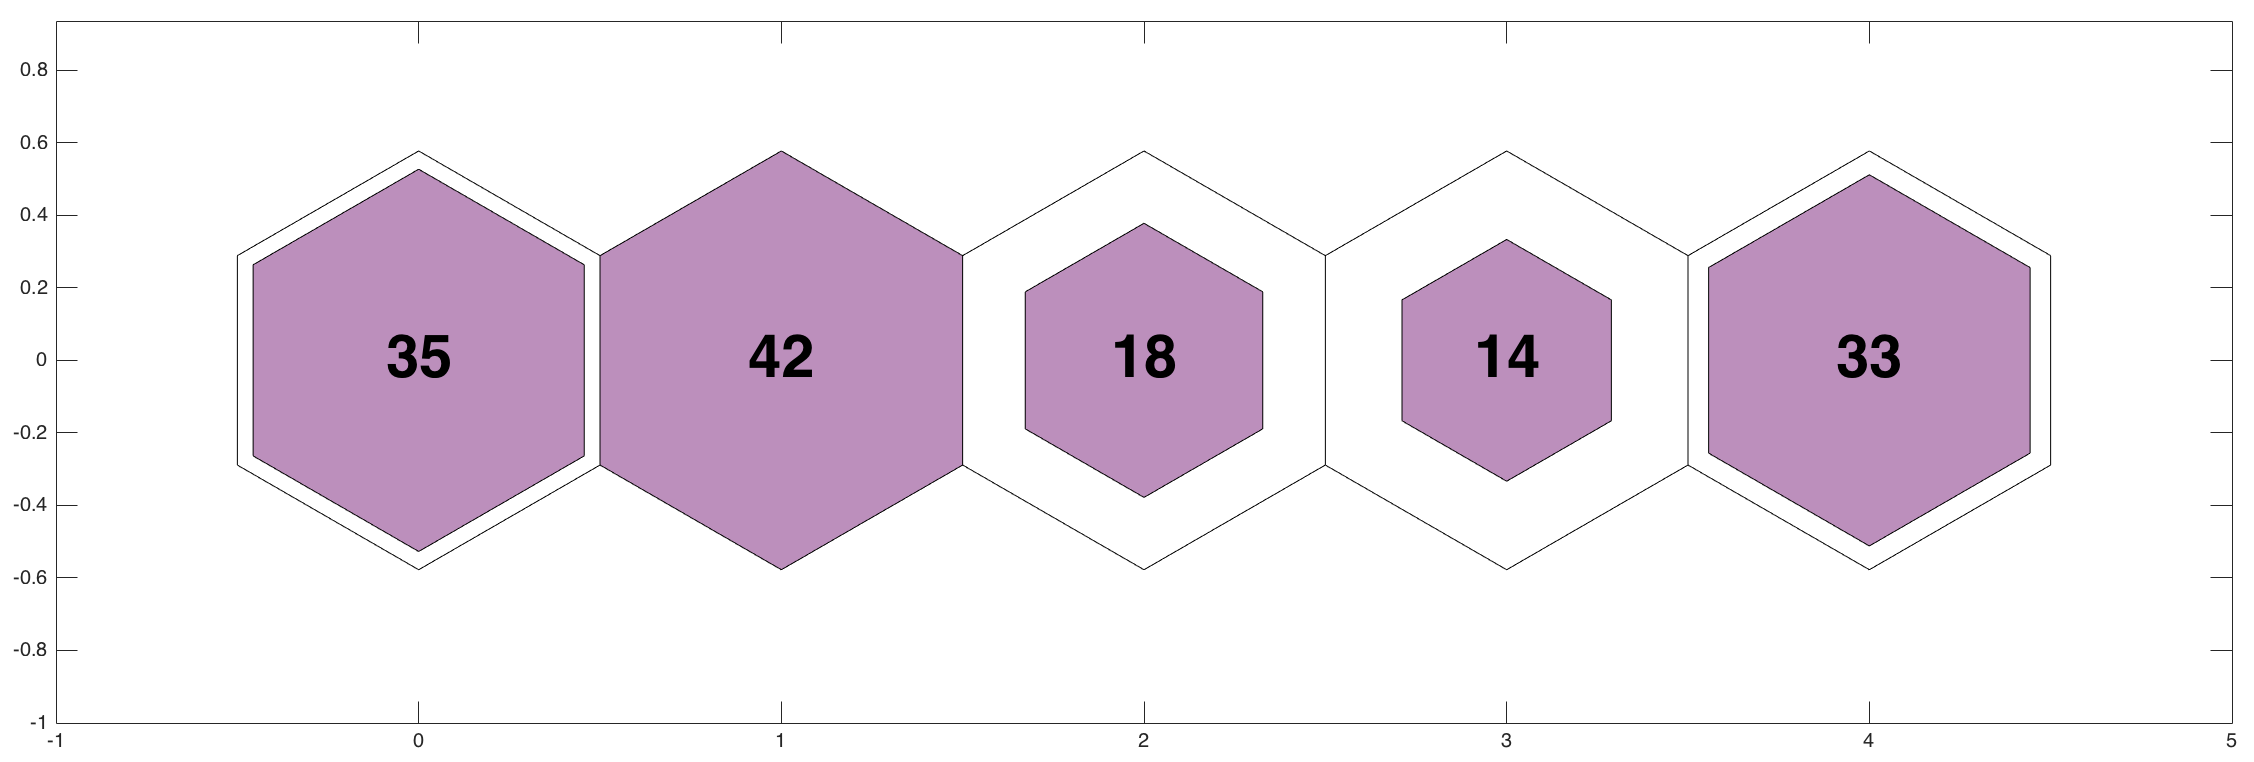
\includegraphics[width=\textwidth]{../images0.01/1d/apps/hit_v_1_by_5.png}
             %\caption{$1\times5$ hits map}
             %\label{fig: 1by5Thits}
        \end{subfigure}
                \caption{Results of training network in $1\times5$~grid.}
         \label{fig: 1by5T}
    \end{figure}
    
    \begin{figure}
        \begin{subfigure}[b]{0.5\textwidth}
            \centering
            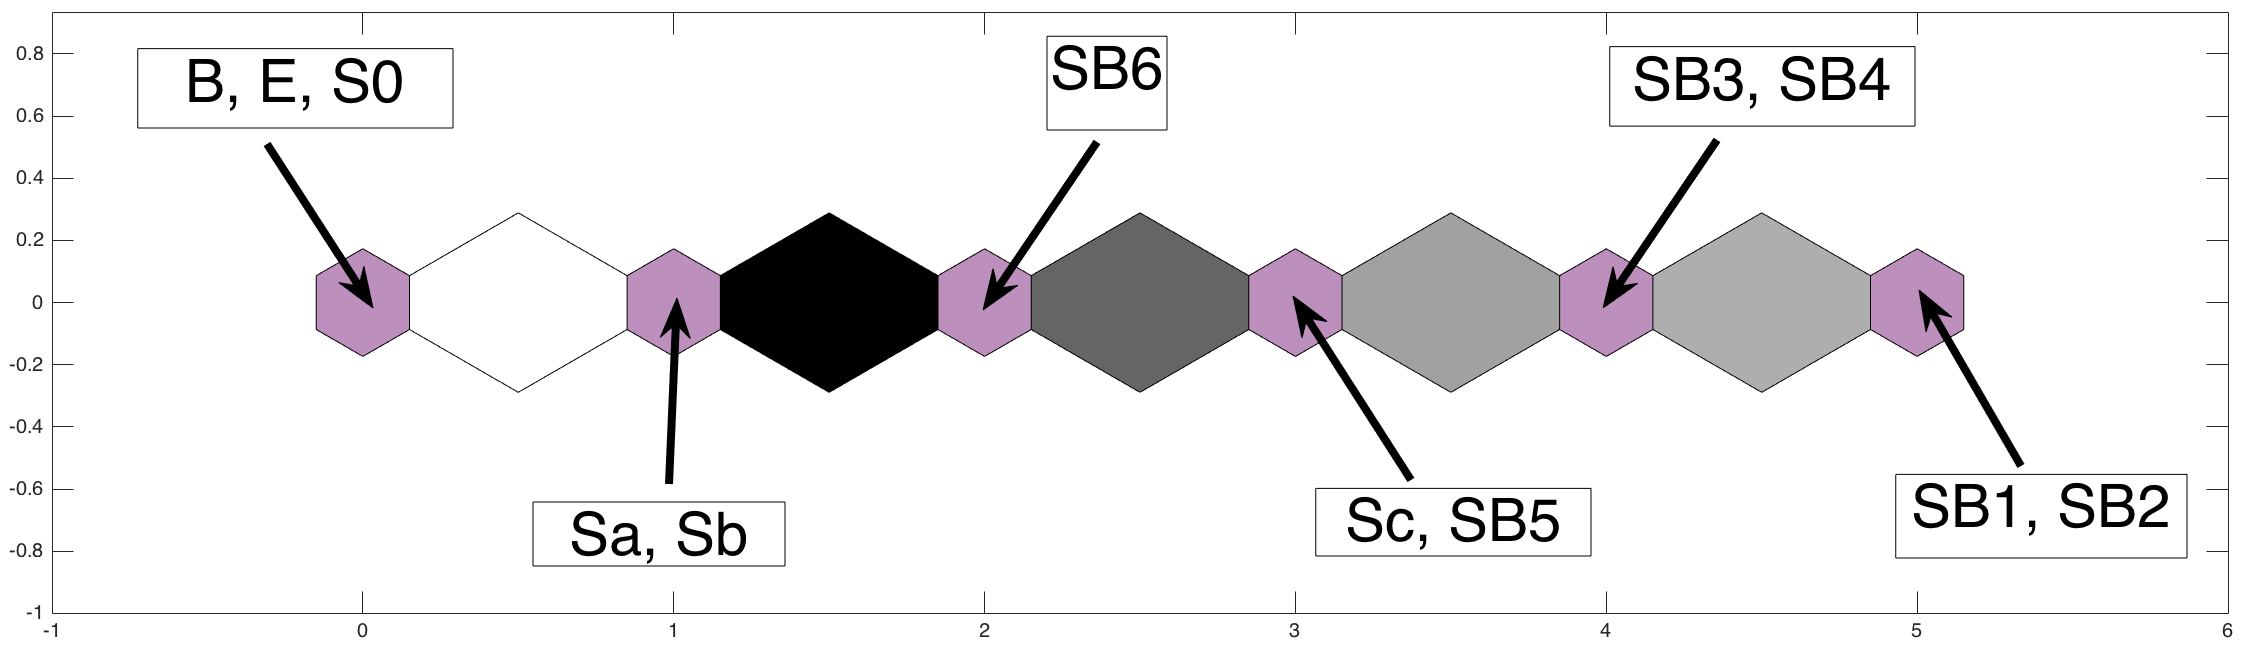
\includegraphics[width=\textwidth]{../images0.01/1d/apps/dist_1_by_6.png}
            %\caption{$1\times6$ weight map}
             %\label{fig: 1by6T}
        \end{subfigure}
        \hfill
        \begin{subfigure}[b]{0.5\textwidth}
             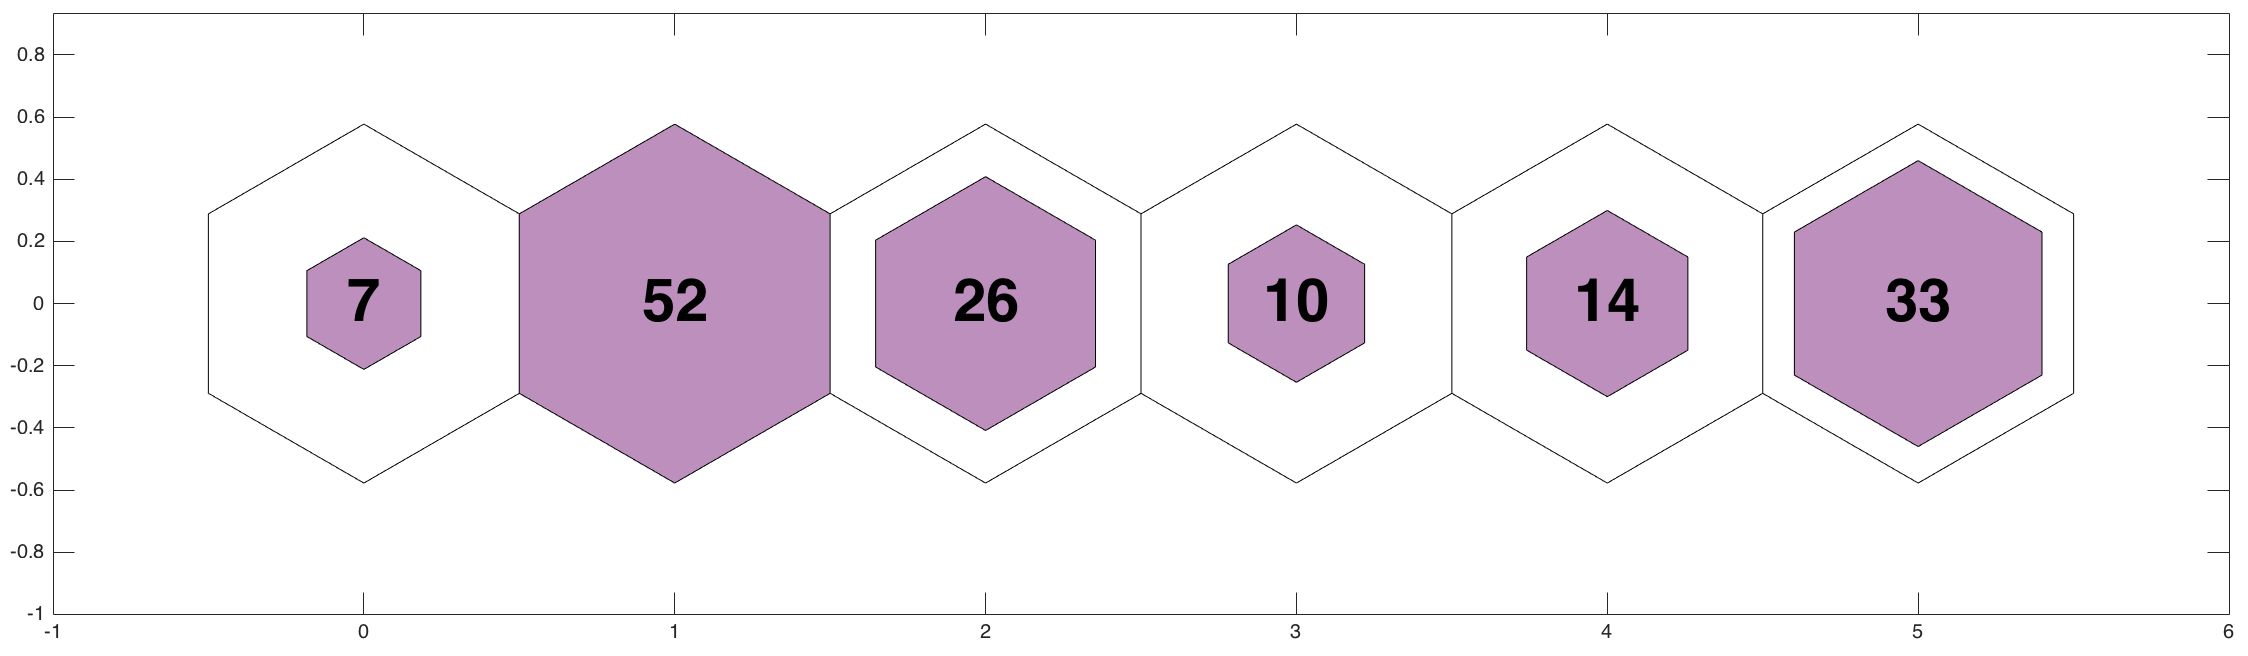
\includegraphics[width=\textwidth]{../images0.01/1d/apps/hit_v_1_by_6.png}
             %\caption{$1\times6$ hits map}
             %\label{fig: 1by6Thits}
        \end{subfigure}
                \caption{Results of training network in $1\times6$~grid.}
         \label{fig: 1by6T}
    \end{figure}
    
    \begin{figure}
        \begin{subfigure}[b]{0.5\textwidth}
            \centering
            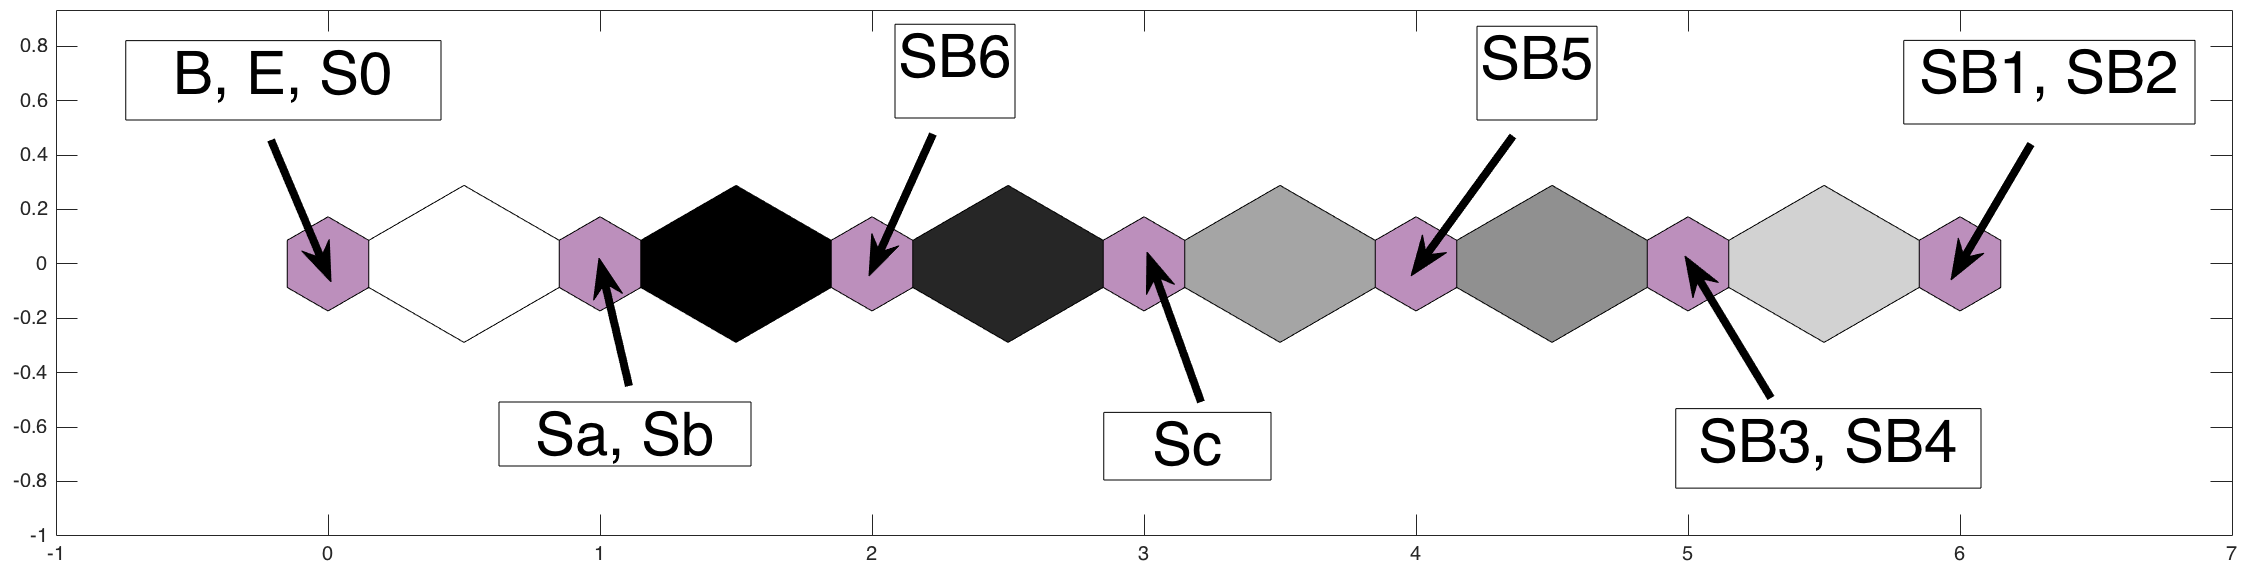
\includegraphics[width=\textwidth]{../images0.01/1d/apps/dist_1_by_7.png}
            %\caption{$1\times7$ weight map}
             %\label{fig: 1by7T}
        \end{subfigure}
        \hfill
        \begin{subfigure}[b]{0.5\textwidth}
             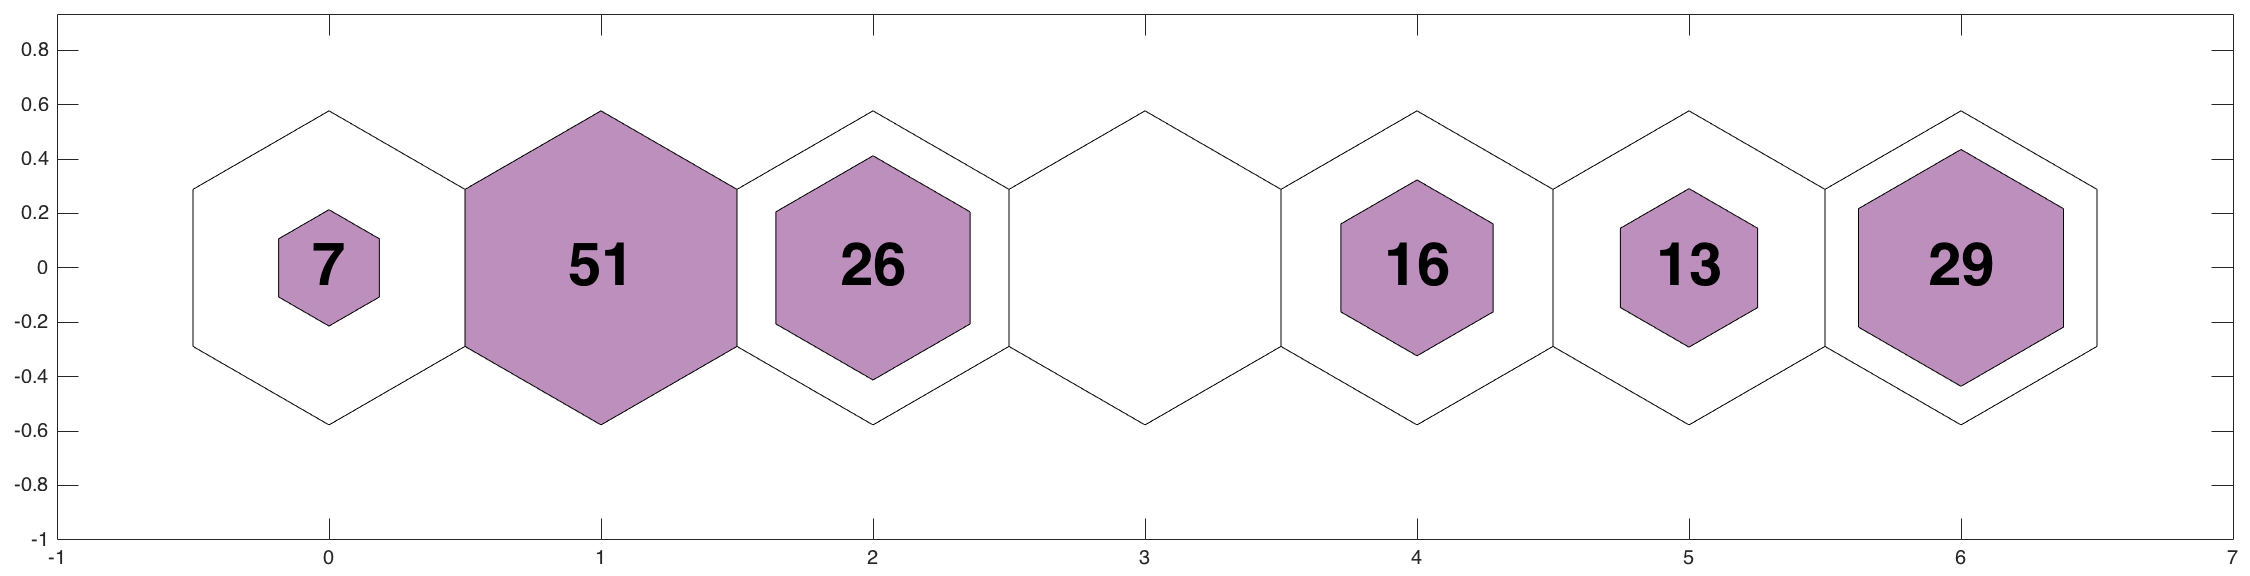
\includegraphics[width=\textwidth]{../images0.01/1d/apps/hit_v_1_by_7.png}
             %\caption{$1\times7$ hits map}
             %\label{fig: 1by7Thits}
        \end{subfigure}
                \caption{Results of training network in $1\times7$~grid.}
         \label{fig: 1by7T}
    \end{figure}
    
    \begin{figure}
        \begin{subfigure}[b]{0.5\textwidth}
            \centering
            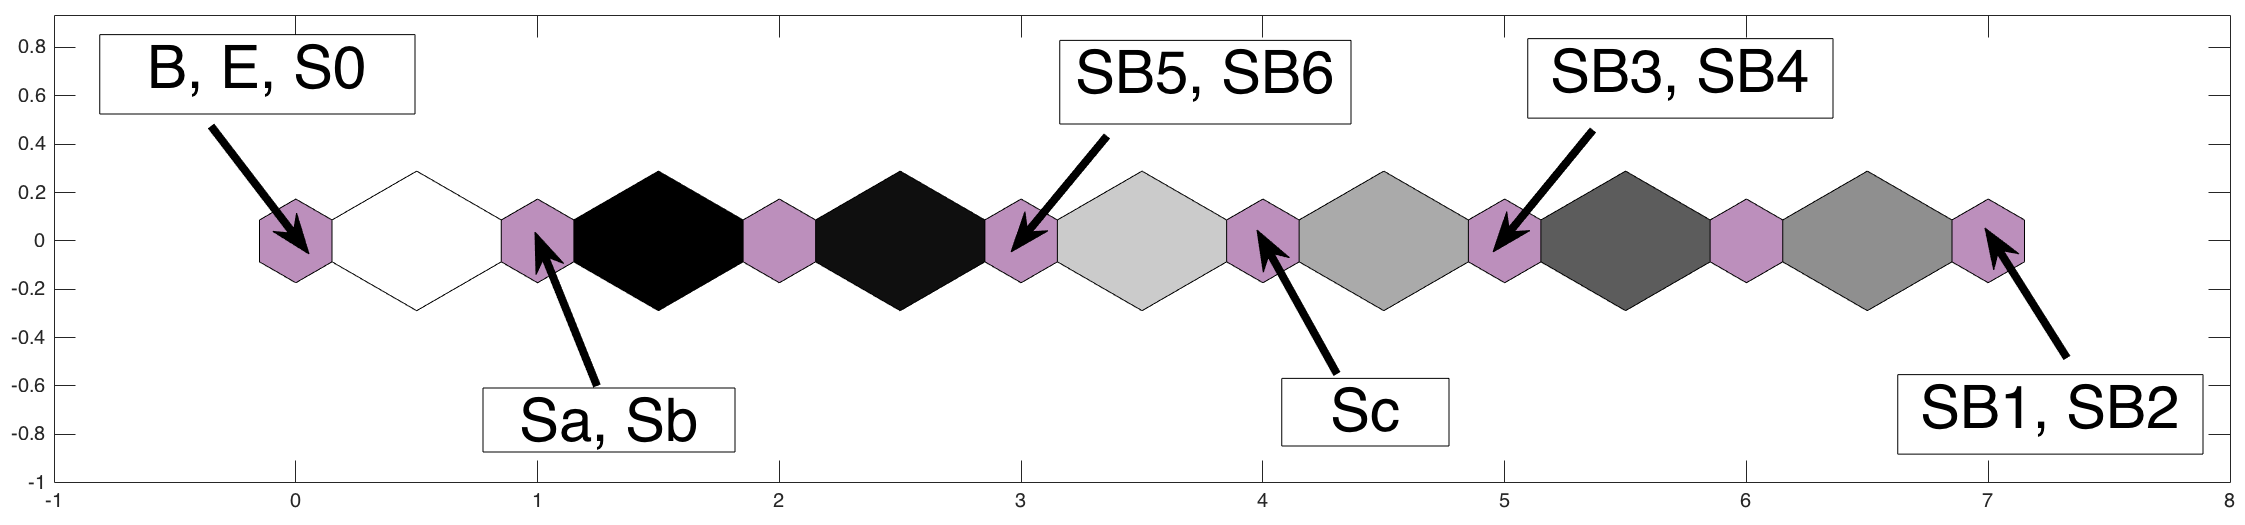
\includegraphics[width=\textwidth]{../images0.01/1d/apps/dist_1_by_8.png}
            %\caption{$1\times8$ weight map}
             %\label{fig: 1by8T}
        \end{subfigure}
        \hfill
        \begin{subfigure}[b]{0.5\textwidth}
             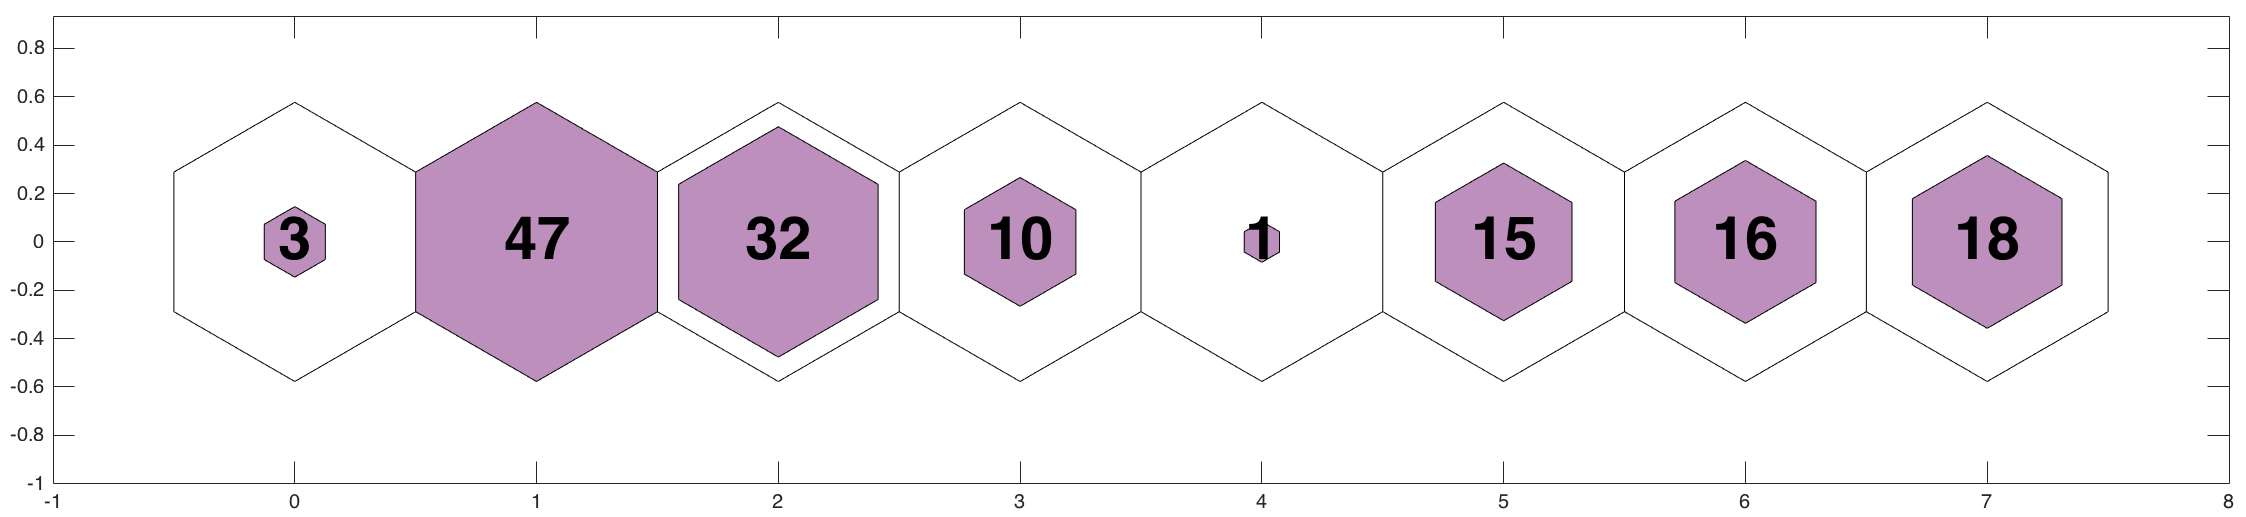
\includegraphics[width=\textwidth]{../images0.01/1d/apps/hit_v_1_by_8.png}
             %\caption{$1\times8$ hits map}
             %\label{fig: 1by8Thits}
        \end{subfigure}
                \caption{Results of training network in $1\times8$~grid.}
         \label{fig: 1by8T}
    \end{figure}
    
    \begin{figure}
        \begin{subfigure}[b]{0.5\textwidth}
            \centering
            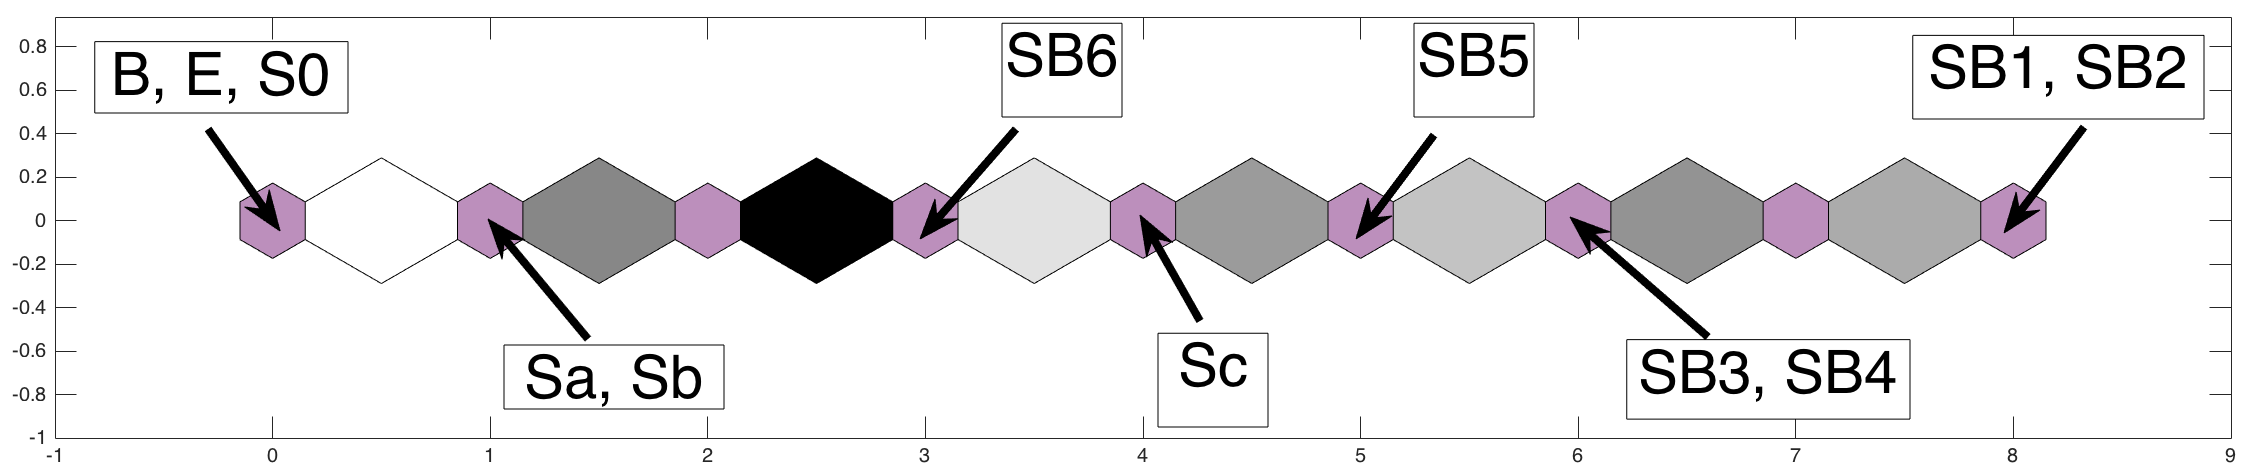
\includegraphics[width=\textwidth]{../images0.01/1d/apps/dist_1_by_9.png}
            %\caption{$1\times9$ weight map}
             %\label{fig: 1by9T}
        \end{subfigure}
        \hfill
        \begin{subfigure}[b]{0.5\textwidth}
             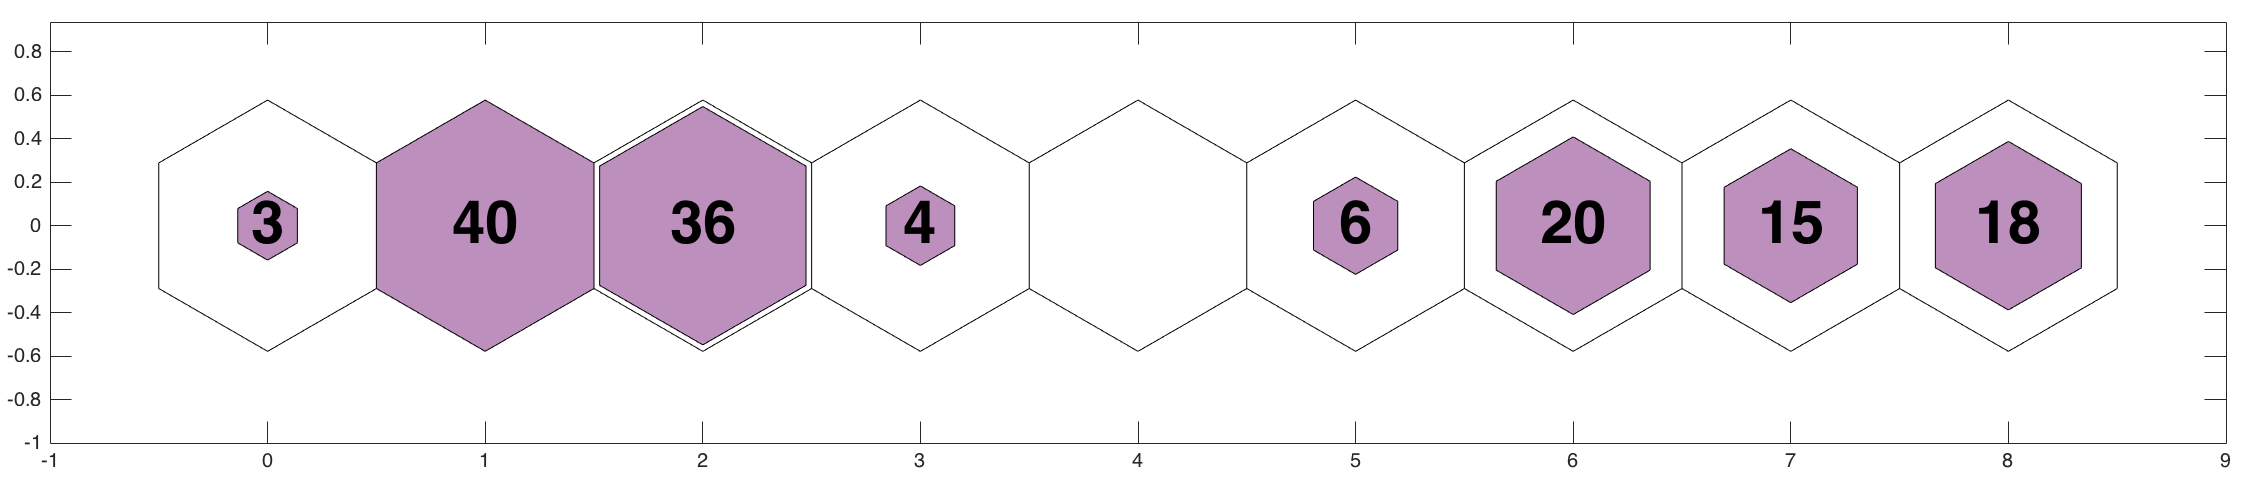
\includegraphics[width=\textwidth]{../images0.01/1d/apps/hit_v_1_by_9.png}
             %\caption{$1\times9$ hits map}
             %\label{fig: 1by9Thits}
        \end{subfigure}
                \caption{Results of training network in $1\times9$~grid.}
         \label{fig: 1by9T}
    \end{figure}

    \begin{figure}
        \begin{subfigure}[b]{0.5\textwidth}
            \centering
            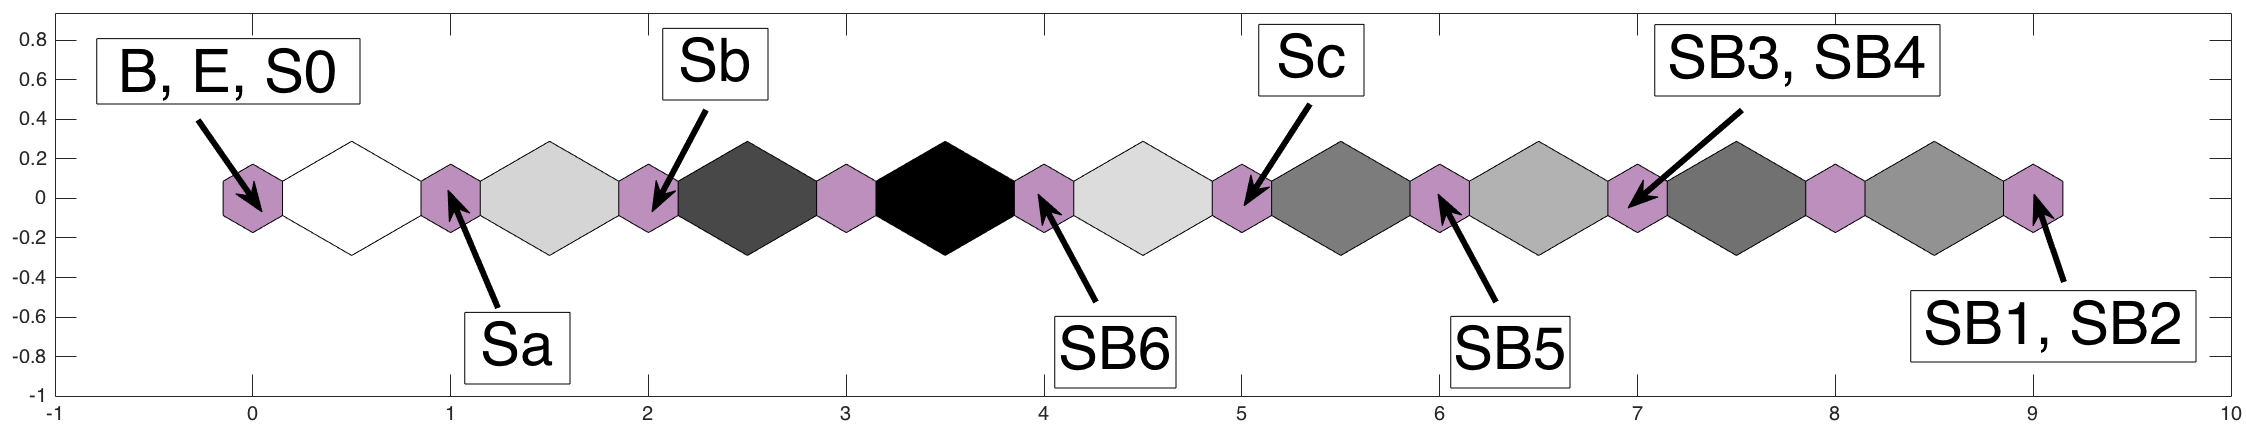
\includegraphics[width=\textwidth,height=2.5cm]{../images0.01/1d/apps/dist_1_by_10.png}
            %\caption{$1\times10$ weight map}
             %\label{fig: 1by10T}
        \end{subfigure}
        \hfill
        \begin{subfigure}[b]{0.5\textwidth}
             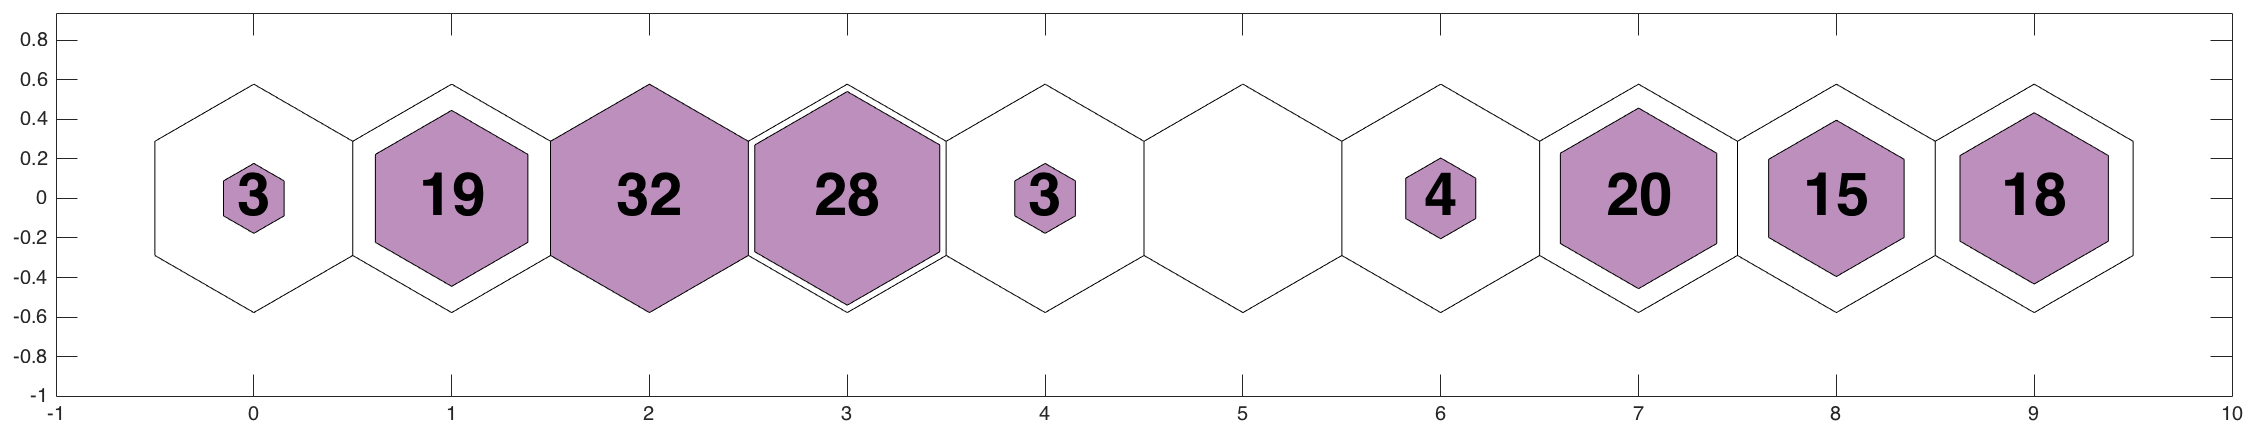
\includegraphics[width=\textwidth,height=2.5cm]{../images0.01/1d/apps/hit_v_1_by_10.png}
             %\caption{$1\times10$ hits map}
             %\label{fig: 1by10Thits}
        \end{subfigure}
                \caption{Results of training network in $1\times10$~grid.}
         \label{fig: 1by10T}
    \end{figure}

    \begin{figure}
        \begin{subfigure}[b]{0.5\textwidth}
            \centering
            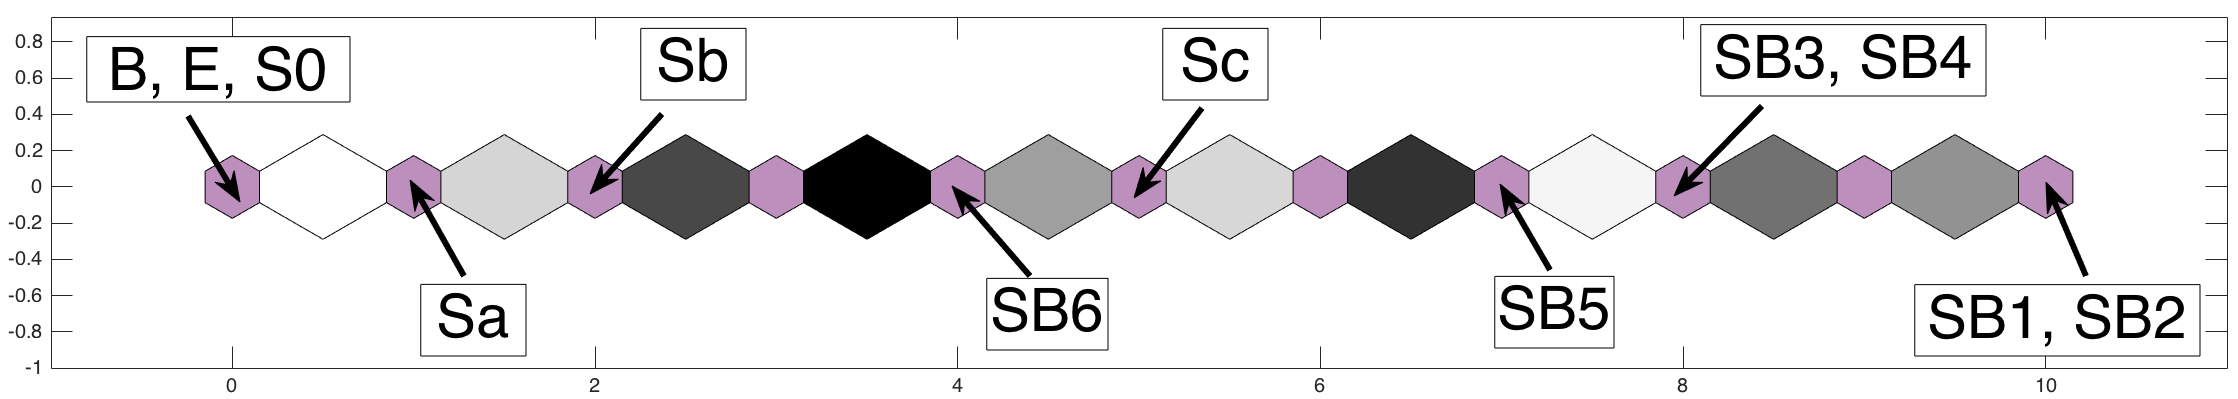
\includegraphics[width=\textwidth,height=2.5cm]{../images0.01/1d/apps/dist_1_by_11.png}
            %\caption{$1\times11$ weight map}
             %\label{fig: 1by11T}
        \end{subfigure}
        \hfill
        \begin{subfigure}[b]{0.5\textwidth}
             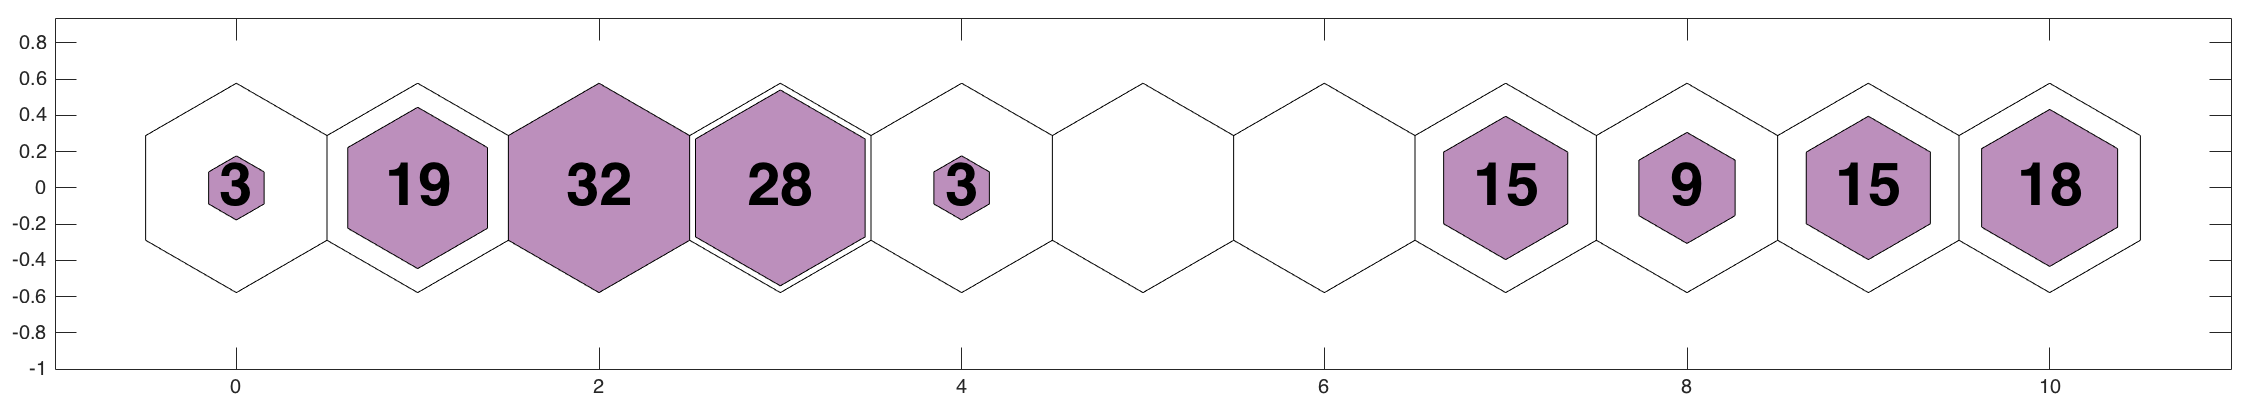
\includegraphics[width=\textwidth,height=2.5cm]{../images0.01/1d/apps/hit_v_1_by_11.png}
             %\caption{$1\times11$ hits map}
             %\label{fig: 1by11Thits}
        \end{subfigure}
                \caption{Results of training network in $1\times11$~grid.}
         \label{fig: 1by11T}
    \end{figure}
    

    \begin{figure}
        \begin{subfigure}[b]{0.5\textwidth}
            \centering
            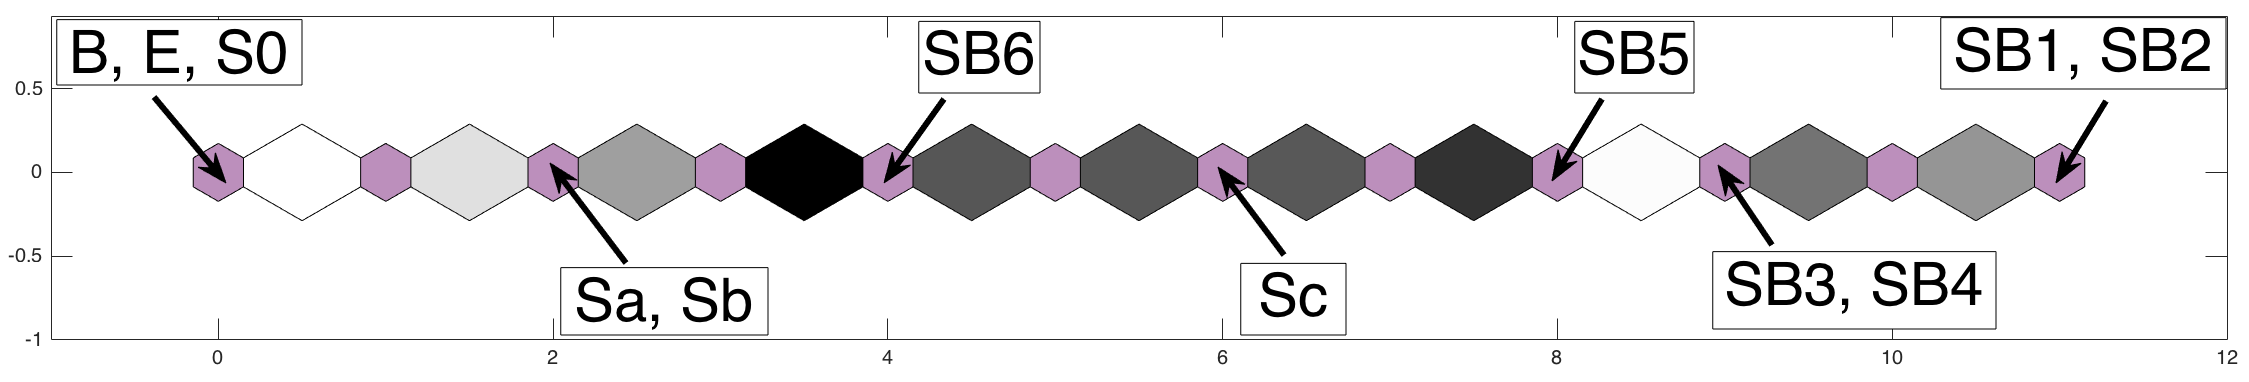
\includegraphics[width=\textwidth,height=2.5cm]{../images0.01/1d/apps/dist_1_by_12.png}
            %\caption{$1\times12$ weight map}
             %\label{fig: 1by12T}
        \end{subfigure}
        \hfill
        \begin{subfigure}[b]{0.5\textwidth}
             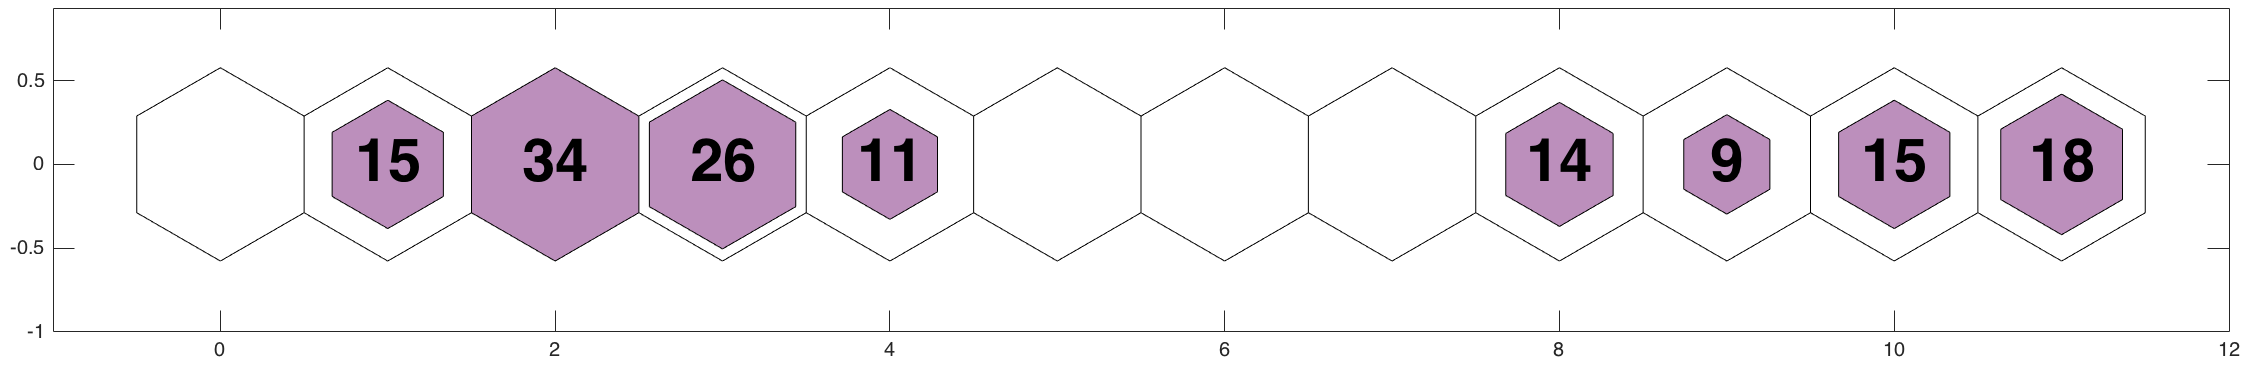
\includegraphics[width=\textwidth,height=2.5cm]{../images0.01/1d/apps/hit_v_1_by_12.png}
             %\caption{$1\times12$ hits map}
             %\label{fig: 1by12Thits}
        \end{subfigure}
                \caption{Results of training network in $1\times12$~grid.}
         \label{fig: 1by12T}
    \end{figure}

    \begin{figure}
        \begin{subfigure}[b]{0.5\textwidth}
            \centering
            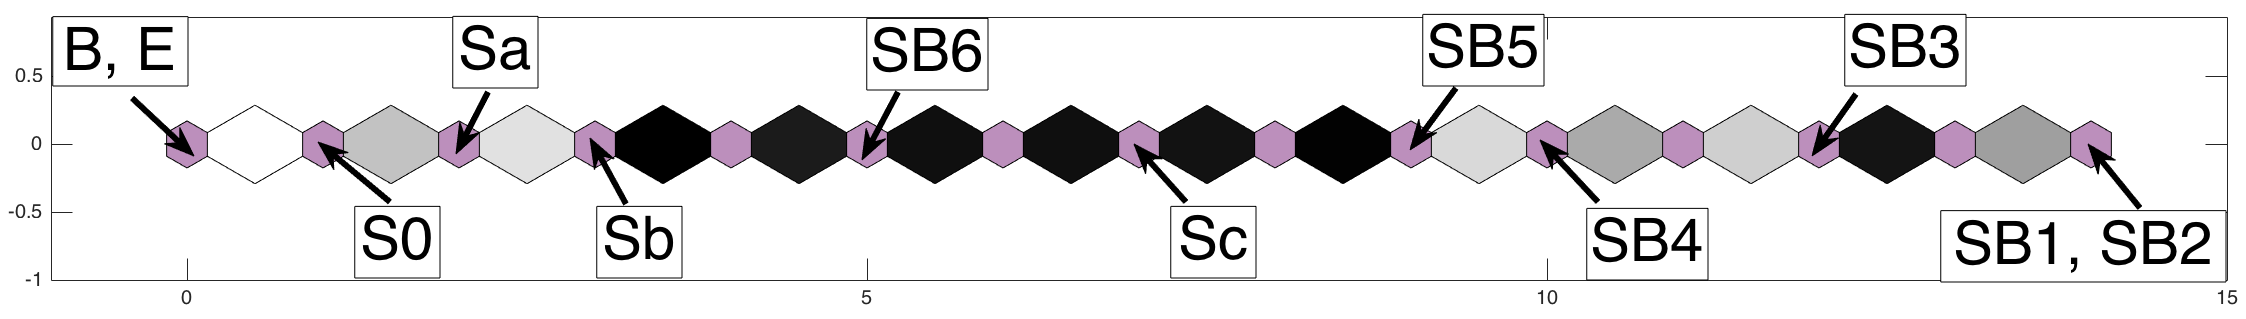
\includegraphics[width=\textwidth,height=2.5cm]{../images0.01/1d/apps/dist_1_by_15.png}
            %\caption{$1\times15$ weight map}
             %\label{fig: 1by15T}
        \end{subfigure}
        \hfill
        \begin{subfigure}[b]{0.5\textwidth}
             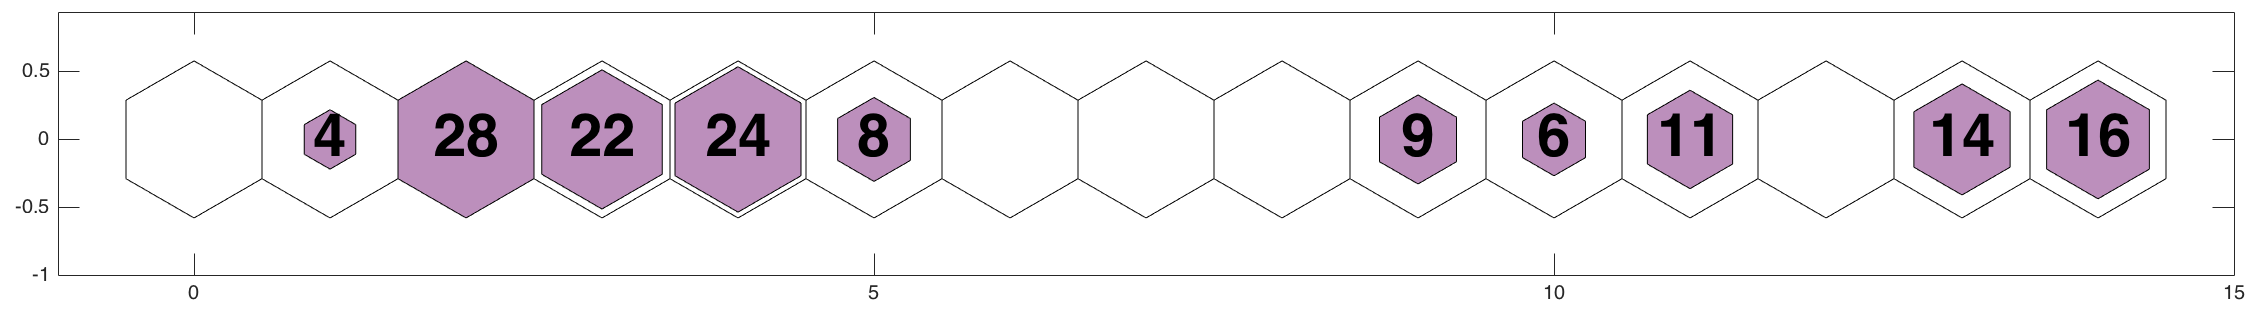
\includegraphics[width=\textwidth,height=2.5cm]{../images0.01/1d/apps/hit_v_1_by_15.png}
             %\caption{$1\times15$ hits map}
             %\label{fig: 1by15Thits}
        \end{subfigure}
                \caption{Results of training network in $1\times15$~grid.}
         \label{fig: 1by15T}
    \end{figure}

    \begin{figure}
        \begin{subfigure}[b]{0.5\textwidth}
            \centering
            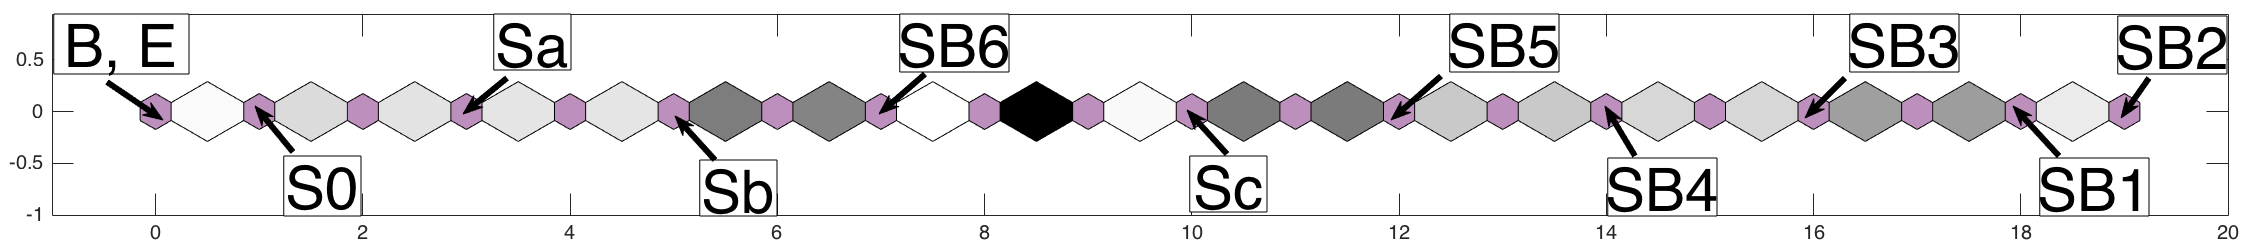
\includegraphics[width=\textwidth,height=2.5cm]{../images0.01/1d/apps/dist_1_by_20.png}
            %\caption{$1\times20$ weight map}
             %\label{fig: 1by20T}
        \end{subfigure}
        \hfill
        \begin{subfigure}[b]{0.5\textwidth}
             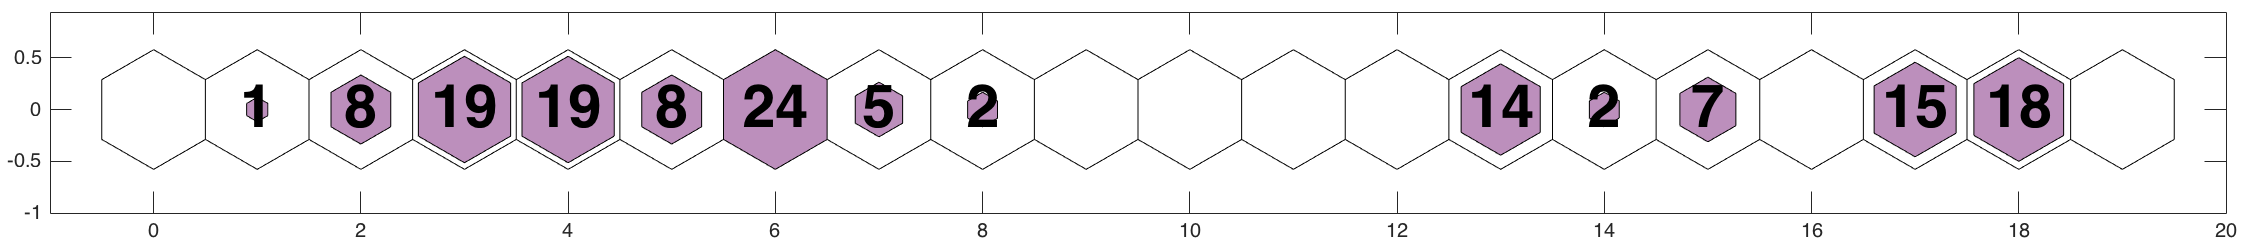
\includegraphics[width=\textwidth,height=2.5cm]{../images0.01/1d/apps/hit_v_1_by_20.png}
             %\caption{$1\times20$ hits map}
             %\label{fig: 1by20Thits}
        \end{subfigure}
                \caption{Results of training network in $1\times20$~grid.}
         \label{fig: 1by20T}
    \end{figure}
    

\newpage



%\subsection{Comparison of the self-organizing maps and K-means methods}
% \label{app: high_Z_1d_k-means}


% In this section we present the results of applying K-means clustering method on the the spectra of 142 galaxies from \citetalias{Hossein12}.
% K-means clustering and SOMs are two of the main unsupervised methods used in astronomical studies \citep[e.g.][]{DAbrusco12, Aycha16}.
% In the K-means methods, the user decides in advance on a number of clusters, $K$. 
% The algorithm randomly chooses $K$ random points to be set as the centroids of the clusters.
% Then it finds the data points that are closest to the each assumed centroid and clusters them together.
% Mean values of the data points assigned to each cluster are calculated and become the new centroid of the cluster. 
% The algorithm finds new clusters based on the new centroids and repeats the procedure until it converges.
% We used \textsc{matlab} K-means library to perform the K-means clustering. %PB: can you give a reference and/or version number? Should do this where you talk about the SOM packages too.

% %K-means vs. SOM
%  In SOM approach a neighborhood function has an important role in the operation of the SOM. 
%  When the radius of the neighbourhood function goes to zero, the algorithm will lose its ordering power and will be reduced to the k-means algorithm.
%  In fact, SOM is a combination of K-means and considering the effect of the neighbors which can be ‘controlled’ by the neighborhood functions (i.e., smoothing process). 
%  In this way, and using a network, SOM maps can find more details.
%  Although a 1-D SOM map can provide a big picture of clustering problems, however, because of smoothing processes even this 1-D map can have a better performance than K-means clustering.

% %The number of clusters in the K-means method is arbitrary and is set by the user.
% % We performed K-means clustering on the \citetalias{Kinney96} template spectra using 4 clusters and on the \citetalias{Hossein12} 142 sample galaxies using 22 clusters.
% In this case we can easily compare the results of K-means clustering with 1D SOMs. 
% To compare the results, we computed the median spectrum for each cluster (in K-means) or neuron (in SOM).
% To classify the 142 sample galaxies, we calculate the median of the spectra in each cluster, and compare them with the \citetalias{Kinney96} template spectra.
% We measured the spectral angle distance between the medians and the template spectra to find the best match between them as follows: %PB: spectral angle distance needs a ref, and a justification - why use something different here compared to for SOM?
% \begin{equation}
%     \cos(\theta) = \frac{\sum_{i=1}^{n} s_it_i}{(\sum_{i=1}^{n} s^2_i)^{0.5} (\sum_{i=1}^{n} t^2_i)^{0.5}}
% \end{equation}
% where $s_i$ and $t_i$ are the $i^{\rm th}$ wavelength of the sample and template spectra, respectively. 
% $\theta$ is the angle between the spectrum, such that a value of zero means completely similar and a value of $180^{\circ}$ means completely different spectra. Since $-1<\cos(\theta)<1$, $1-\cos(\theta)$ is an easier way to measure and report the dissimilarity between two spectra.
% A \citetalias{Kinney96} template spectrum that has the most similarity with the median spectrum of a cluster would be assigned to the all galaxies in the cluster. %PB: I don't quite understand this sentence.
 

% \begin{figure*}
%                 \begin{subfigure}[b]{0.49\textwidth}
%                     \centering
%                   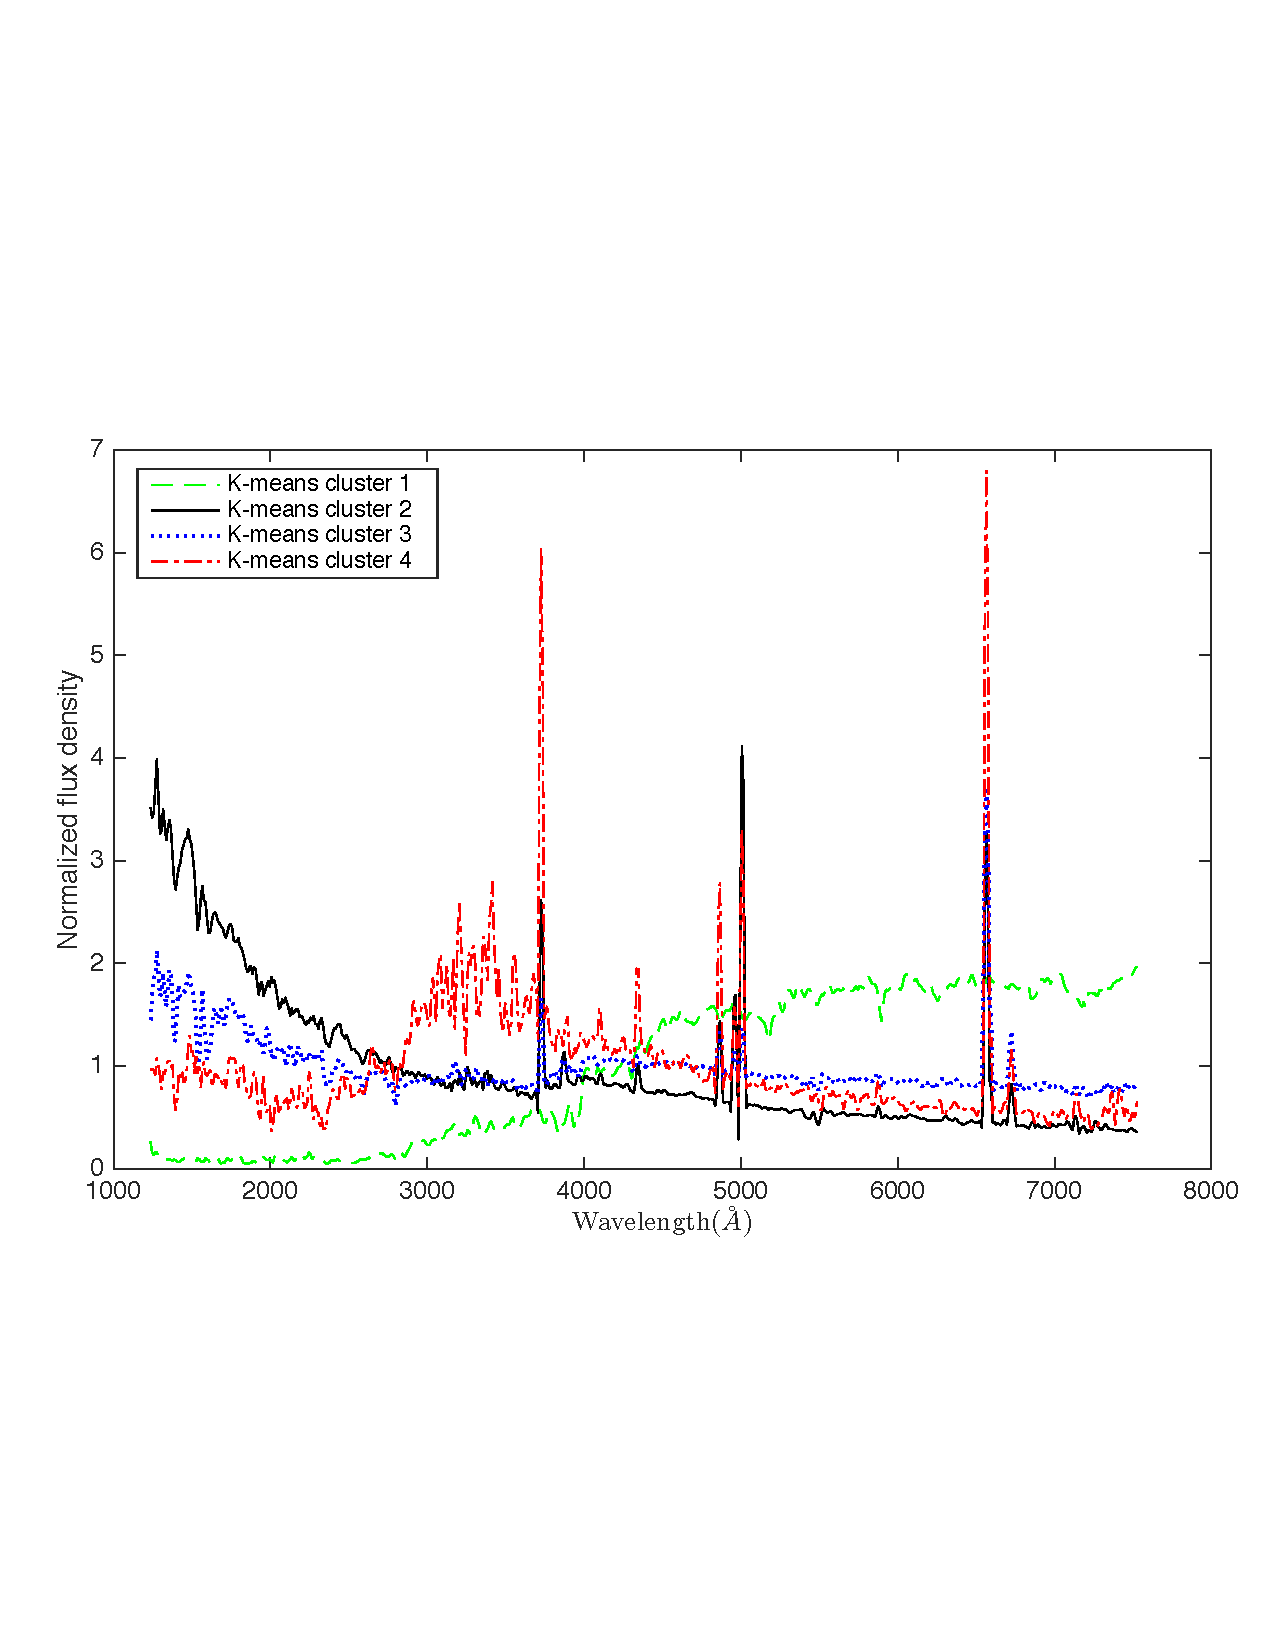
\includegraphics[width=.99\textwidth, height= 7.5cm]{k_means_images/classified_group_in_4cluster.pdf}
%                 \end{subfigure}
%                 \hfill
%                 \begin{subfigure}[b]{0.49\textwidth}
%                     \centering 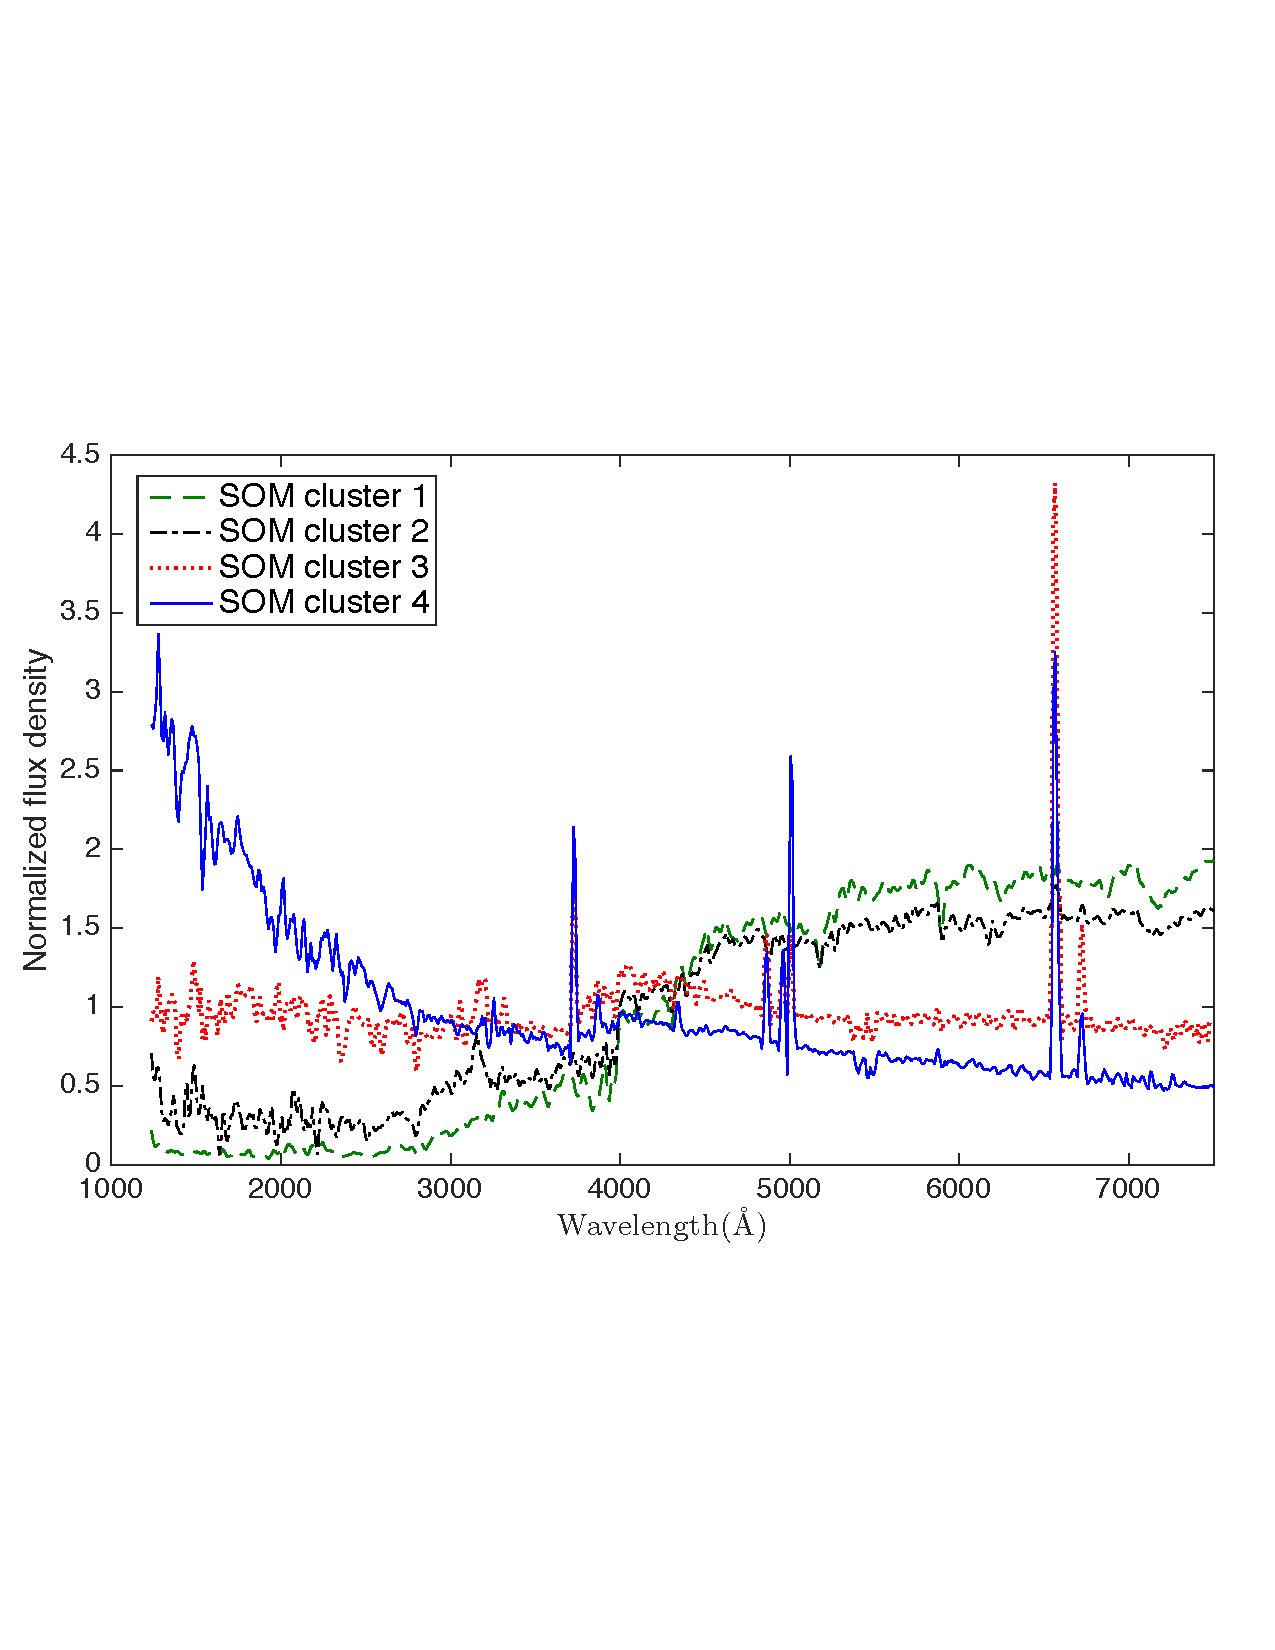
\includegraphics[width=.99\textwidth, height= 7.5cm]{k_means_images/classified_group_in_4cluster_som.pdf}
%                 \end{subfigure}
%                 \caption{Clustering the \citetalias{Kinney96} template spectra using K-means clustering (left) and SOM (right). Note that both methods randomly assign the initial values for their analysis, therefore the cluster number is only used for distinguishing cluster membership.}
%                  \label{fig: som_k_means_4}
% \end{figure*}
% Fig.~\ref{fig: som_k_means_4} shows the clustering of the template spectra in 4 groups using both K-means and SOMs.
% In the K-means method there are no empty clusters, hence a $K=12$ clustering would produce one-object clusters as in Fig.~\ref{fig: k96}.
% Both plots in Fig.~\ref{fig: som_k_means_4} separated the most starburst and quiescent galaxies in a similar manner.
% However, they show discrepancies for spectral types between the extreme cases. 
% The other difference between these two methods is that the network created by the SOM method can be used to classify the other spectra, while for the K-means clusters they can only be used for one set of data.



% \begin{figure*}
%                 \begin{subfigure}[b]{0.49\textwidth}
%                     \centering
%                   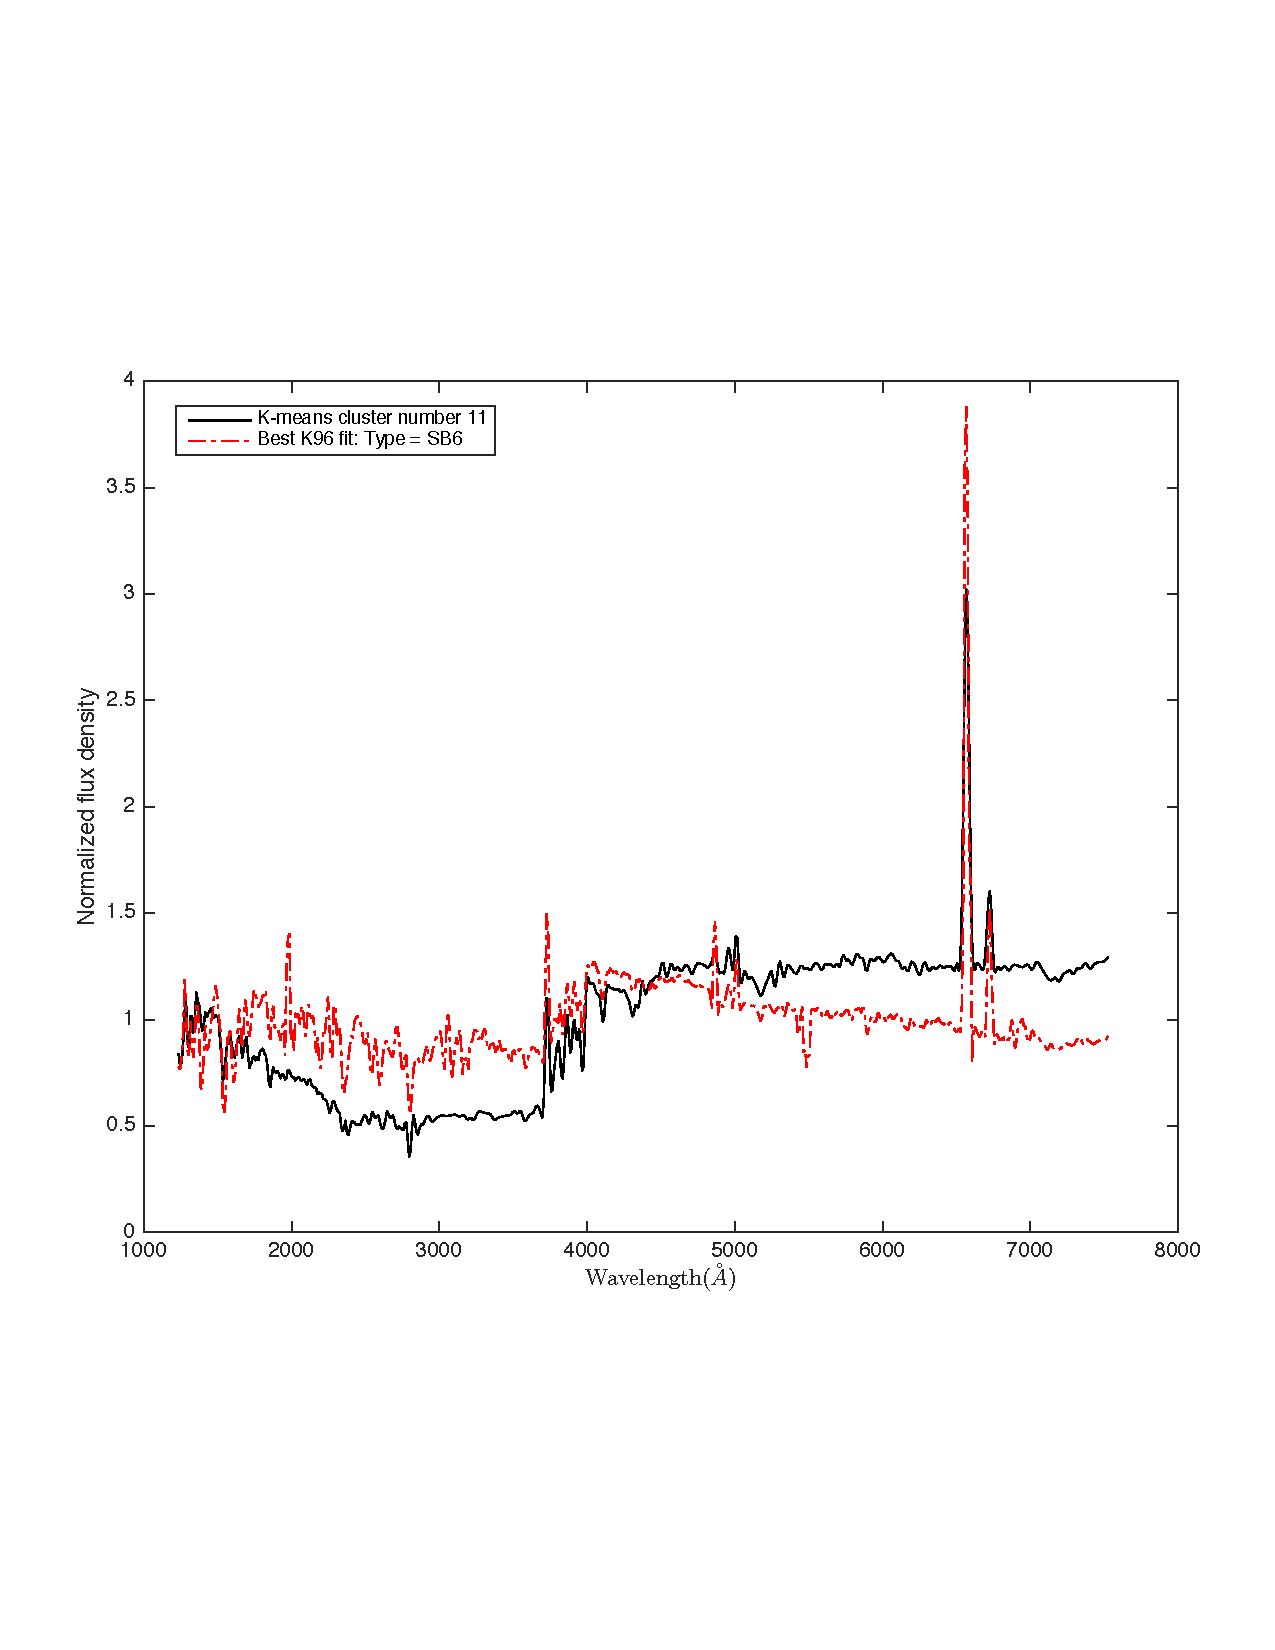
\includegraphics[width=.99\textwidth, height= 7.5cm]{k_means_images/max_cosine2.pdf}
%                 \end{subfigure}
%                 \hfill
%                 \begin{subfigure}[b]{0.49\textwidth}
%                     \centering 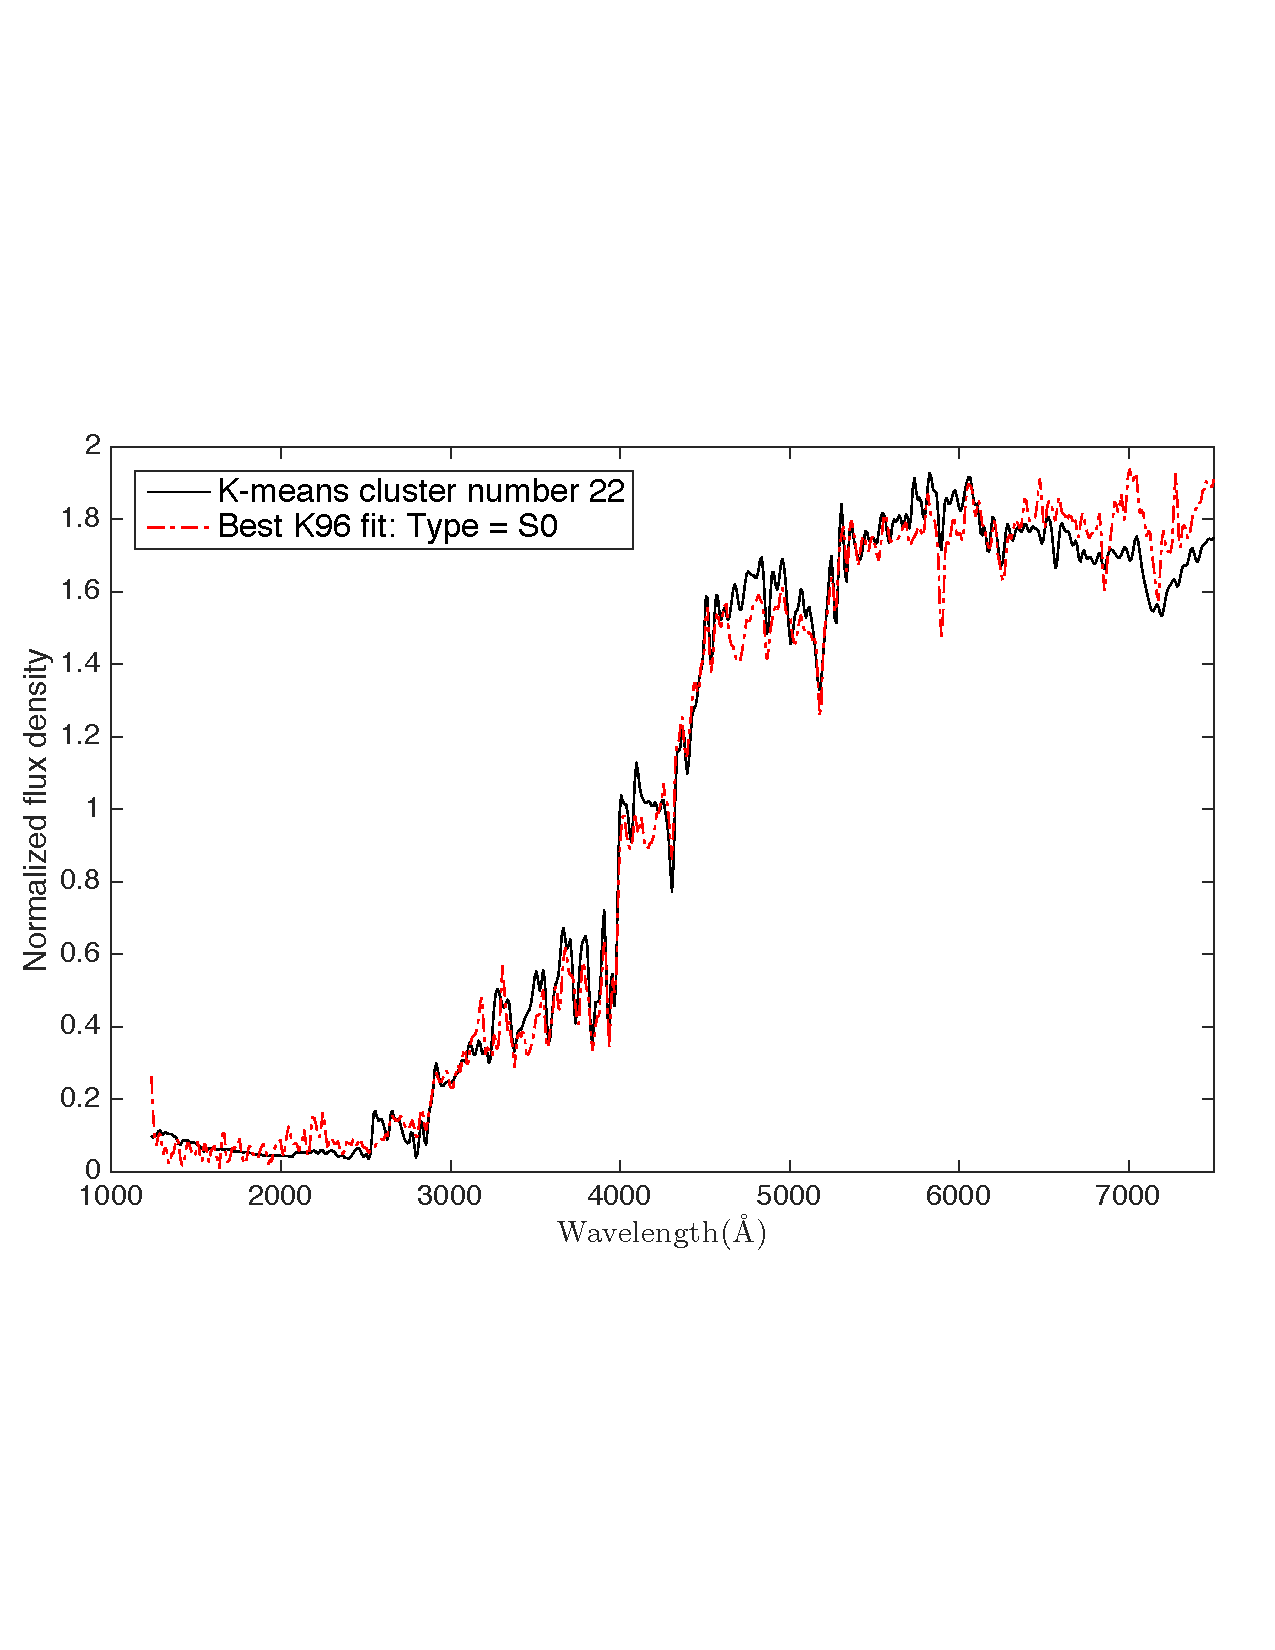
\includegraphics[width=.99\textwidth, height= 7.5cm]{k_means_images/min_cosine2.pdf}
%                 \end{subfigure}
%                 \caption{Left: the best-matched of the \citetalias{Kinney96} templates for the median spectrum of members in cluster number 11. This fit has the maximum $1-\cos(\theta)$ among all 22 clusters. Right: the best fit of the \citetalias{Kinney96} templates to the median spectrum of cluster number 17. This the best fitting result for 22 clusters.}
%                  \label{fig: k_means_minmax}
% \end{figure*}
% For analyzing 142 sample galaxies from \citetalias{Hossein12}, we chose the number of clusters for the K-means analysis to be 22.
% The median spectra of the members of each cluster were fitted by a spectrum from the \citetalias{Kinney96} templates.
% Although the K-means clustering method separated the spectra of 142 sample galaxies into 22 different groups, only 7 of the template spectra were best matches with these 22 groups (some of the groups are classified as the same spectral type).
% %As it is clear in Fig.~\ref{fig: k_means_minmax}, in some cases even the most similar template spectra is not a good fit to the median spectra of the clusters.
% Fig.~\ref{fig: k_means_minmax} shows the best and the worst fitting results among the 22 clusters. 
% As we expected from the results of Section~\ref{sec: 1Dv} and \citetalias{Hossein12} paper, we cannot classify all the 142 sample galaxies with exactly 12 templates. 
% Some of the classifications are almost perfect matches, and there are group of galaxies that are close to but not exactly the same as any of the template spectra.
% The right plot in the Fig.~\ref{fig: k_means_minmax} is an example of group of galaxies that can not be considered as an outlier (in the sense that they are not a completely different type of galaxies), but they cannot be matched exactly with any of the template spectra.

% %PB: this paragraph seems oddly placed here since it's not really about K-means
% Being limited to the template set is one of the disadvantages of the K-means algorithm over the SOM method. 
% As mentioned in Sections~\ref{sec: 1Dv} and \ref{sec: 2D}, by performing the SOM method on the template spectra, we create networks of neurons which each  either represents one of the spectra from the templates or a spectrum that has (dis-)similarity with any of the template spectra. %PB:  second part of this sentence needs rewording
% We can say that using SOM, we introduced a new template based on the \citetalias{Kinney96} template spectra, and classified the 142 sample galaxies based on this new template. %PB: too many uses of "template" in this sentence?

% There are substantial differences between the K-means and SOM-based classification.
% From the K-means clustering, we classified 5 out of 22 clusters, 42 galaxies in total, as Sa type galaxies; 7 clusters, 28 galaxies in total, were classified as SB1 type galaxies.
% Using the SOM method (see Fig.~\ref{fig: 1by22V}, only 19 galaxies were classified as Sa and 19 galaxies were classified as SB1. 
% Fig.~\ref{fig: som_k_means_comp} shows the comparison between the median of the spectra classified by SOM and by K-means clustering. 
% The medians from both methods are clearly tracing each other.
% However, the normalized flux in each case is slightly different: 
% the SB1 galaxies are fainter at short wavelengths and brighter at longer wavelengths for the K-means clusters compared to the SOM ones.
% These differences are reversed for Sa galaxies.
% Using K-means clustering, no clusters were classified as Sb or SB2, which have very similar spectra to Sa and SB1, respectively.
% On the other hand, using the SOM method, 14 galaxies were recognized as having similar spectra to SB2, and 33 galaxies were recognized to have spectra similar to Sa or Sb.
% The differences in the classification and ignoring the templates with similar spectra might come from the error in K-means clustering or error in fitting problem. % PB: need to reword this sentence but I don't understand it.
% In either case we can conclude that SOM method classifies galaxies considering more details than K-means clustering method. %PB: not sure I see how you come to this conclusion




% \begin{figure*}
%                 \begin{subfigure}[b]{0.49\textwidth}
%                     \centering
%                   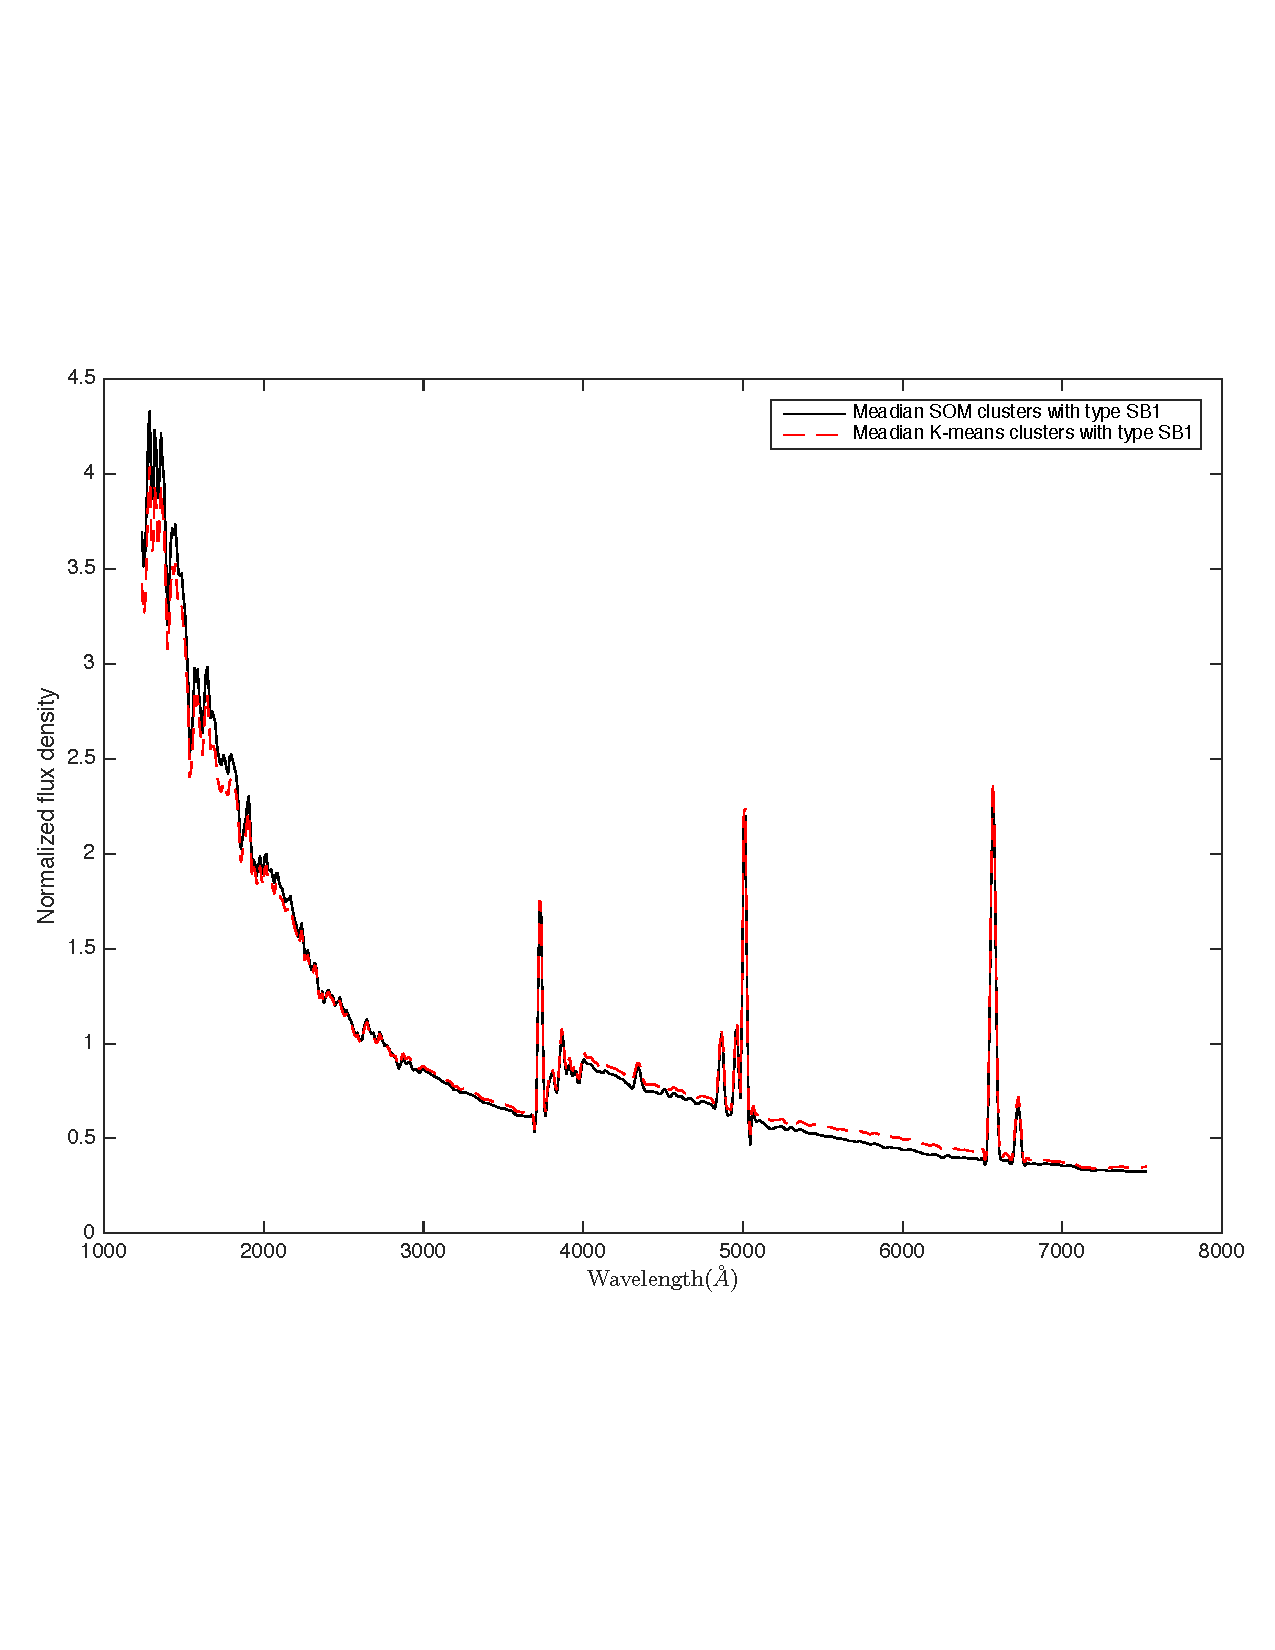
\includegraphics[width=0.99\textwidth, height=7.5cm]{k_means_images/SB1_comp.pdf}
%                 \end{subfigure}
%                 \hfill
%                 \begin{subfigure}[b]{0.49\textwidth}
%                     \centering 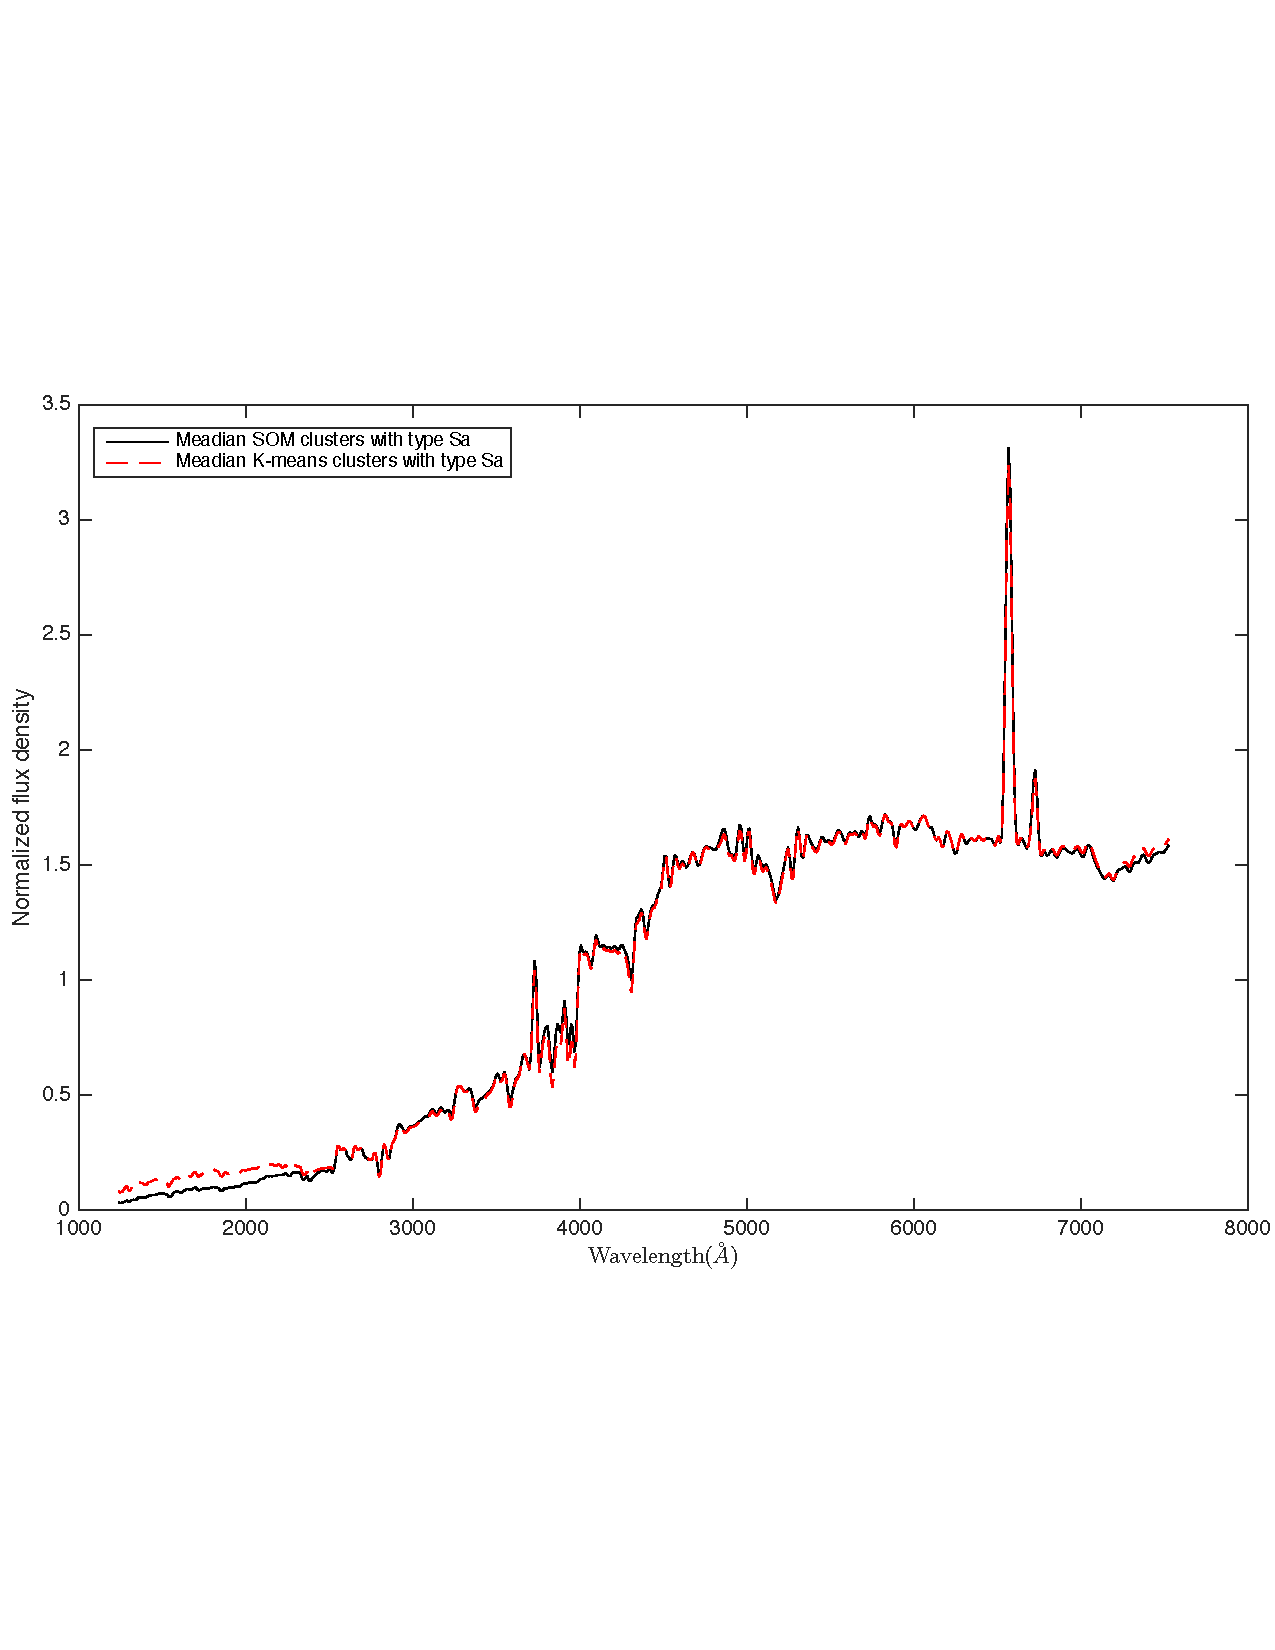
\includegraphics[width=\textwidth, height= 7.2cm]{k_means_images/Sa_comp.pdf}
%                 \end{subfigure}
%                 \caption{Comparing median of classified clusters from the K-means (dashed red lines) and SOM (solid black lines) methods. Left: the clusters in both methods classified as SB1. Right: the clusters in both methods  classified as Sa.}
%                  \label{fig: som_k_means_comp}
% \end{figure*}

